% =============================================================
% 7 Анализ упорного подшипника скольжения
% =============================================================
\chapter{Анализ рельефного упорного подшипника скольжения}

\section{Объект исследования и исходные данные}

Объектом исследования в настоящей главе является упорный подшипник
скольжения с секторными колодками~\cite{gropper2018,wasilczuk2008}. Неподвижные колодки удерживают
осевую нагрузку вращающегося диска (ротора). Подшипник состоит
из~$N_{\mathrm{pads}} = 6$ одинаковых секторных колодок; расчёт
ведётся для одного сектора с последующим пересчётом интегральных
характеристик на полный подшипник.

В отличие от радиального подшипника (главы~5 и~6), где несущая сила
обусловлена эксцентриситетом цапфы, в упорном подшипнике давление
возникает вследствие клинового зазора между колодкой и диском.
Основным геометрическим параметром является параметр клина
$K = h_{\mathrm{in}} / h_{\mathrm{out}}$, где
$h_{\mathrm{in}}$~-- зазор на входной кромке сектора,
$h_{\mathrm{out}}$~-- зазор на выходной кромке.
Характер уравнения Рейнольдса также отличается: задача формулируется
в цилиндрических координатах $(r, \theta)$, а скорость скольжения
зависит от радиуса: $U(r) = \omega \cdot r$~\cite{brajdic2005,heinrichson2008}.

Основные параметры подшипника сведены в
таблицу~\ref{tab:thrust_params}.

\begin{table}[!ht]
\centering
\caption{Параметры упорного подшипника скольжения}
\label{tab:thrust_params}
\begin{tabularx}{\textwidth}{|X|c|c|c|}
\hline
\multicolumn{1}{|c|}{\textbf{Параметр}} & \textbf{Обозначение} & \textbf{Значение} & \textbf{Единица} \\
\hline
Внутренний радиус          & $R_{\mathrm{in}}$   & 30{,}0  & мм \\
\hline
Наружный радиус            & $R_{\mathrm{out}}$  & 60{,}0  & мм \\
\hline
Число колодок              & $N_{\mathrm{pads}}$ & 6       & -- \\
\hline
Угол сектора               & $\beta = 2\pi/N$    & 60{,}0  & $^{\circ}$ \\
\hline
Минимальный зазор          & $h_{\mathrm{out}}$  & 50      & мкм \\
\hline
Номинальный параметр клина & $K_{\mathrm{nom}}$  & 2{,}0   & -- \\
\hline
Динамическая вязкость      & $\mu$               & 0{,}020 & Па$\cdot$с \\
\hline
Частота вращения           & $n$                 & 3000    & об/мин \\
\hline
Угловая скорость           & $\omega$            & 314{,}2 & рад/с \\
\hline
\end{tabularx}
\end{table}

\FloatBarrier

Схема сектора упорного подшипника представлена на
рисунке~\ref{fig:thrust_scheme}.

\begin{figure}[!ht]
\centering
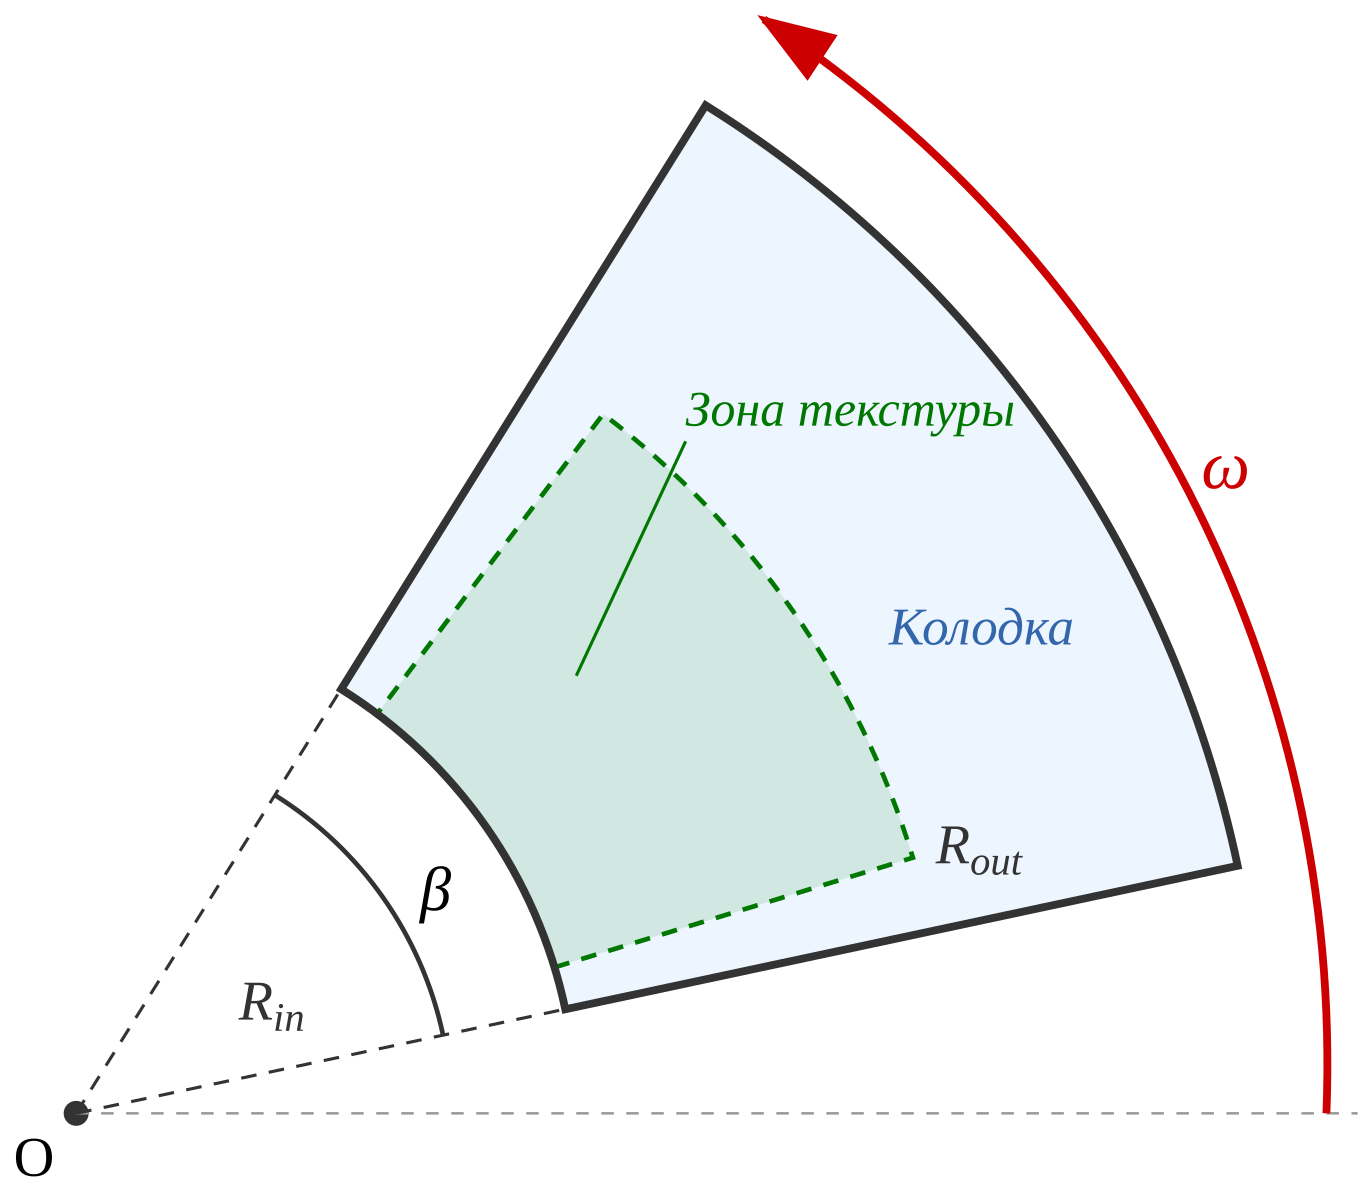
\includegraphics[width=\textwidth,height=0.9\textheight,keepaspectratio]{figures/ch07/fig_7_1.png}
\caption{Расчётная схема сектора упорного подшипника скольжения}
\label{fig:thrust_scheme}
\end{figure}

\FloatBarrier


\section{Расчётная схема и математическая модель}

Расчётная область представляет собой развёртку поверхности одного
сектора: $r \in [R_{\mathrm{in}},\, R_{\mathrm{out}}]$,
$\theta \in [0,\, \beta]$.

Угловая скорость вращения диска определяется частотой вращения:
\begin{equation}
  \omega = \frac{2\pi n}{60}.
  \label{eq:thrust_omega}
\end{equation}
Скорость скольжения на радиусе~$r$:
\begin{equation}
  U(r) = \omega \cdot r.
  \label{eq:thrust_U}
\end{equation}

Толщина смазочного зазора между колодкой и диском определяется
линейным законом клина:
\begin{equation}
  h(r, \theta) = h_{\mathrm{out}}
    + (h_{\mathrm{in}} - h_{\mathrm{out}})
    \left(1 - \frac{\theta}{\beta}\right)
  = h_{\mathrm{out}}
    \left[1 + (K - 1)\left(1 - \frac{\theta}{\beta}\right)\right],
  \label{eq:thrust_h}
\end{equation}
где $K = h_{\mathrm{in}} / h_{\mathrm{out}}$~-- параметр клина
($K > 1$). При $\theta = 0$ (входная кромка) зазор максимален
$h = h_{\mathrm{in}} = K \cdot h_{\mathrm{out}}$; при
$\theta = \beta$ (выходная кромка) зазор минимален
$h = h_{\mathrm{out}}$.

Распределение давления в смазочном слое описывается уравнением
Рейнольдса в цилиндрических координатах:
\begin{equation}
  \frac{\partial}{\partial r}
    \left[r\, h^3\, \frac{\partial p}{\partial r}\right]
  + \frac{\partial}{\partial \theta}
    \left[\frac{h^3}{r}\, \frac{\partial p}{\partial \theta}\right]
  = 6\mu\omega\, r\, \frac{\partial h}{\partial \theta}.
  \label{eq:thrust_reynolds}
\end{equation}

Граничные условия:
\begin{equation}
\left\{\;
\begin{aligned}
  p &= 0 \quad \text{при } \theta = 0
    \quad \text{(входная кромка)}, \\
  p &= 0 \quad \text{при } \theta = \beta
    \quad \text{(выходная кромка)}, \\
  p &= 0 \quad \text{при } r = R_{\mathrm{in}},\;
    r = R_{\mathrm{out}}.
\end{aligned}
\right.
  \label{eq:thrust_bc}
\end{equation}
Условие кавитации: $p \geq 0$.

Условия $p = 0$ на радиальных кромках представляют собой упрощение
модели, принятое для сравнительного анализа гладкого
и текстурированного вариантов на одной и той же расчётной области.

Интегральные характеристики подшипника вычисляются следующим
образом. Несущая сила:
\begin{equation}
  W = N_{\mathrm{pads}} \iint p\, r\, \mathrm{d}r\, \mathrm{d}\theta.
  \label{eq:thrust_W}
\end{equation}
Момент трения (упрощённая оценка; напорная составляющая
не учитывается):
\begin{equation}
  M_f = N_{\mathrm{pads}} \iint
    \frac{\mu\, \omega\, r}{h}\, r^2\,
    \mathrm{d}r\, \mathrm{d}\theta.
  \label{eq:thrust_Mf}
\end{equation}
Средний радиус:
\begin{equation}
  R_m = \frac{2}{3}\,
    \frac{R_{\mathrm{out}}^3 - R_{\mathrm{in}}^3}
         {R_{\mathrm{out}}^2 - R_{\mathrm{in}}^2}.
  \label{eq:thrust_Rm}
\end{equation}
Коэффициент трения:
\begin{equation}
  f_T = \frac{M_f}{W \cdot R_m}.
  \label{eq:thrust_fT}
\end{equation}
Расход смазочного материала:
\begin{equation}
  Q = N_{\mathrm{pads}} \int
    \left(-\frac{h^3}{12\mu}\,
    \frac{\partial p}{\partial r}\right)
    r\, \mathrm{d}\theta
    \bigg|_{r = R_{\mathrm{out}}}.
  \label{eq:thrust_Q}
\end{equation}
Максимальное давление в секторе:
$p_{\max} = \max\limits_{r,\theta} p(r, \theta)$.


\section{Конфигурации детерминированных микроструктур}

Аналогично главам~5 и~6, в качестве элементов рельефа используются
эллипсоидальные лунки~\eqref{eq:profile_ellipsoidal}
с шахматной раскладкой~\eqref{eq:layout_staggered}.
В координатах $(r, \theta)$ добавка от лунки записывается
в виде:
\begin{equation}
  \Delta h = H_p \cdot h_{\mathrm{out}}
    \left(1 - \frac{\Delta r^2}{a_r^2}
    - \frac{\Delta\theta^2}{a_\theta^2}\right)
  \quad \text{при}\quad
    \frac{\Delta r^2}{a_r^2}
    + \frac{\Delta\theta^2}{a_\theta^2} \leq 1,
  \label{eq:thrust_dimple}
\end{equation}
где $a_r$, $a_\theta$~-- полуоси эллипса в направлениях~$r$
и~$\theta$, $H_p$~-- безразмерная глубина лунки, нормированная
на~$h_{\mathrm{out}}$.

Конфигурации T1 и~T2 нанесены в зоне
$\theta \in [0{,}1\beta;\; 0{,}7\beta]$~-- входная и средняя
часть клина, где давление нарастает. Конфигурация~T3 нанесена
в зоне $\theta \in [0{,}3\beta;\; 0{,}9\beta]$~-- средняя
и выходная часть клина.

Ожидается, что текстурирование в зоне нарастания давления (T1,~T2)
эффективнее, чем в зоне спада (T3), поскольку лунки создают
дополнительные гидродинамические клинья именно там, где формируется
основная несущая способность.

Параметры рассматриваемых конфигураций приведены в
таблице~\ref{tab:thrust_texture}.

\begin{table}[!ht]
\centering
\caption{Параметры конфигураций текстуры упорного подшипника}
\label{tab:thrust_texture}
\begin{tabularx}{\textwidth}{|X|c|c|c|c|c|}
\hline
\multicolumn{1}{|c|}{\textbf{Конфигурация}}
  & $\boldsymbol{H_p}$
  & $\boldsymbol{A^*}$
  & $\boldsymbol{B^*}$
  & \textbf{Зона нанесения}
  & \textbf{Число лунок} \\
\hline
T1 & 0{,}20 & 0{,}060 & 0{,}025 & $0{,}1\beta$--$0{,}7\beta$ & $5 \times 8$ \\
\hline
T2 & 0{,}40 & 0{,}060 & 0{,}025 & $0{,}1\beta$--$0{,}7\beta$ & $5 \times 8$ \\
\hline
T3 & 0{,}20 & 0{,}060 & 0{,}025 & $0{,}3\beta$--$0{,}9\beta$ & $5 \times 8$ \\
\hline
\end{tabularx}
\end{table}

\FloatBarrier

Безразмерные полуоси определяются как
$A^* = a_r / (R_{\mathrm{out}} - R_{\mathrm{in}})$,
$B^* = a_\theta / \beta$.

Карта распределения зазора для конфигурации~T2 представлена
на рисунке~\ref{fig:thrust_texture_map}.

\begin{figure}[!ht]
\centering
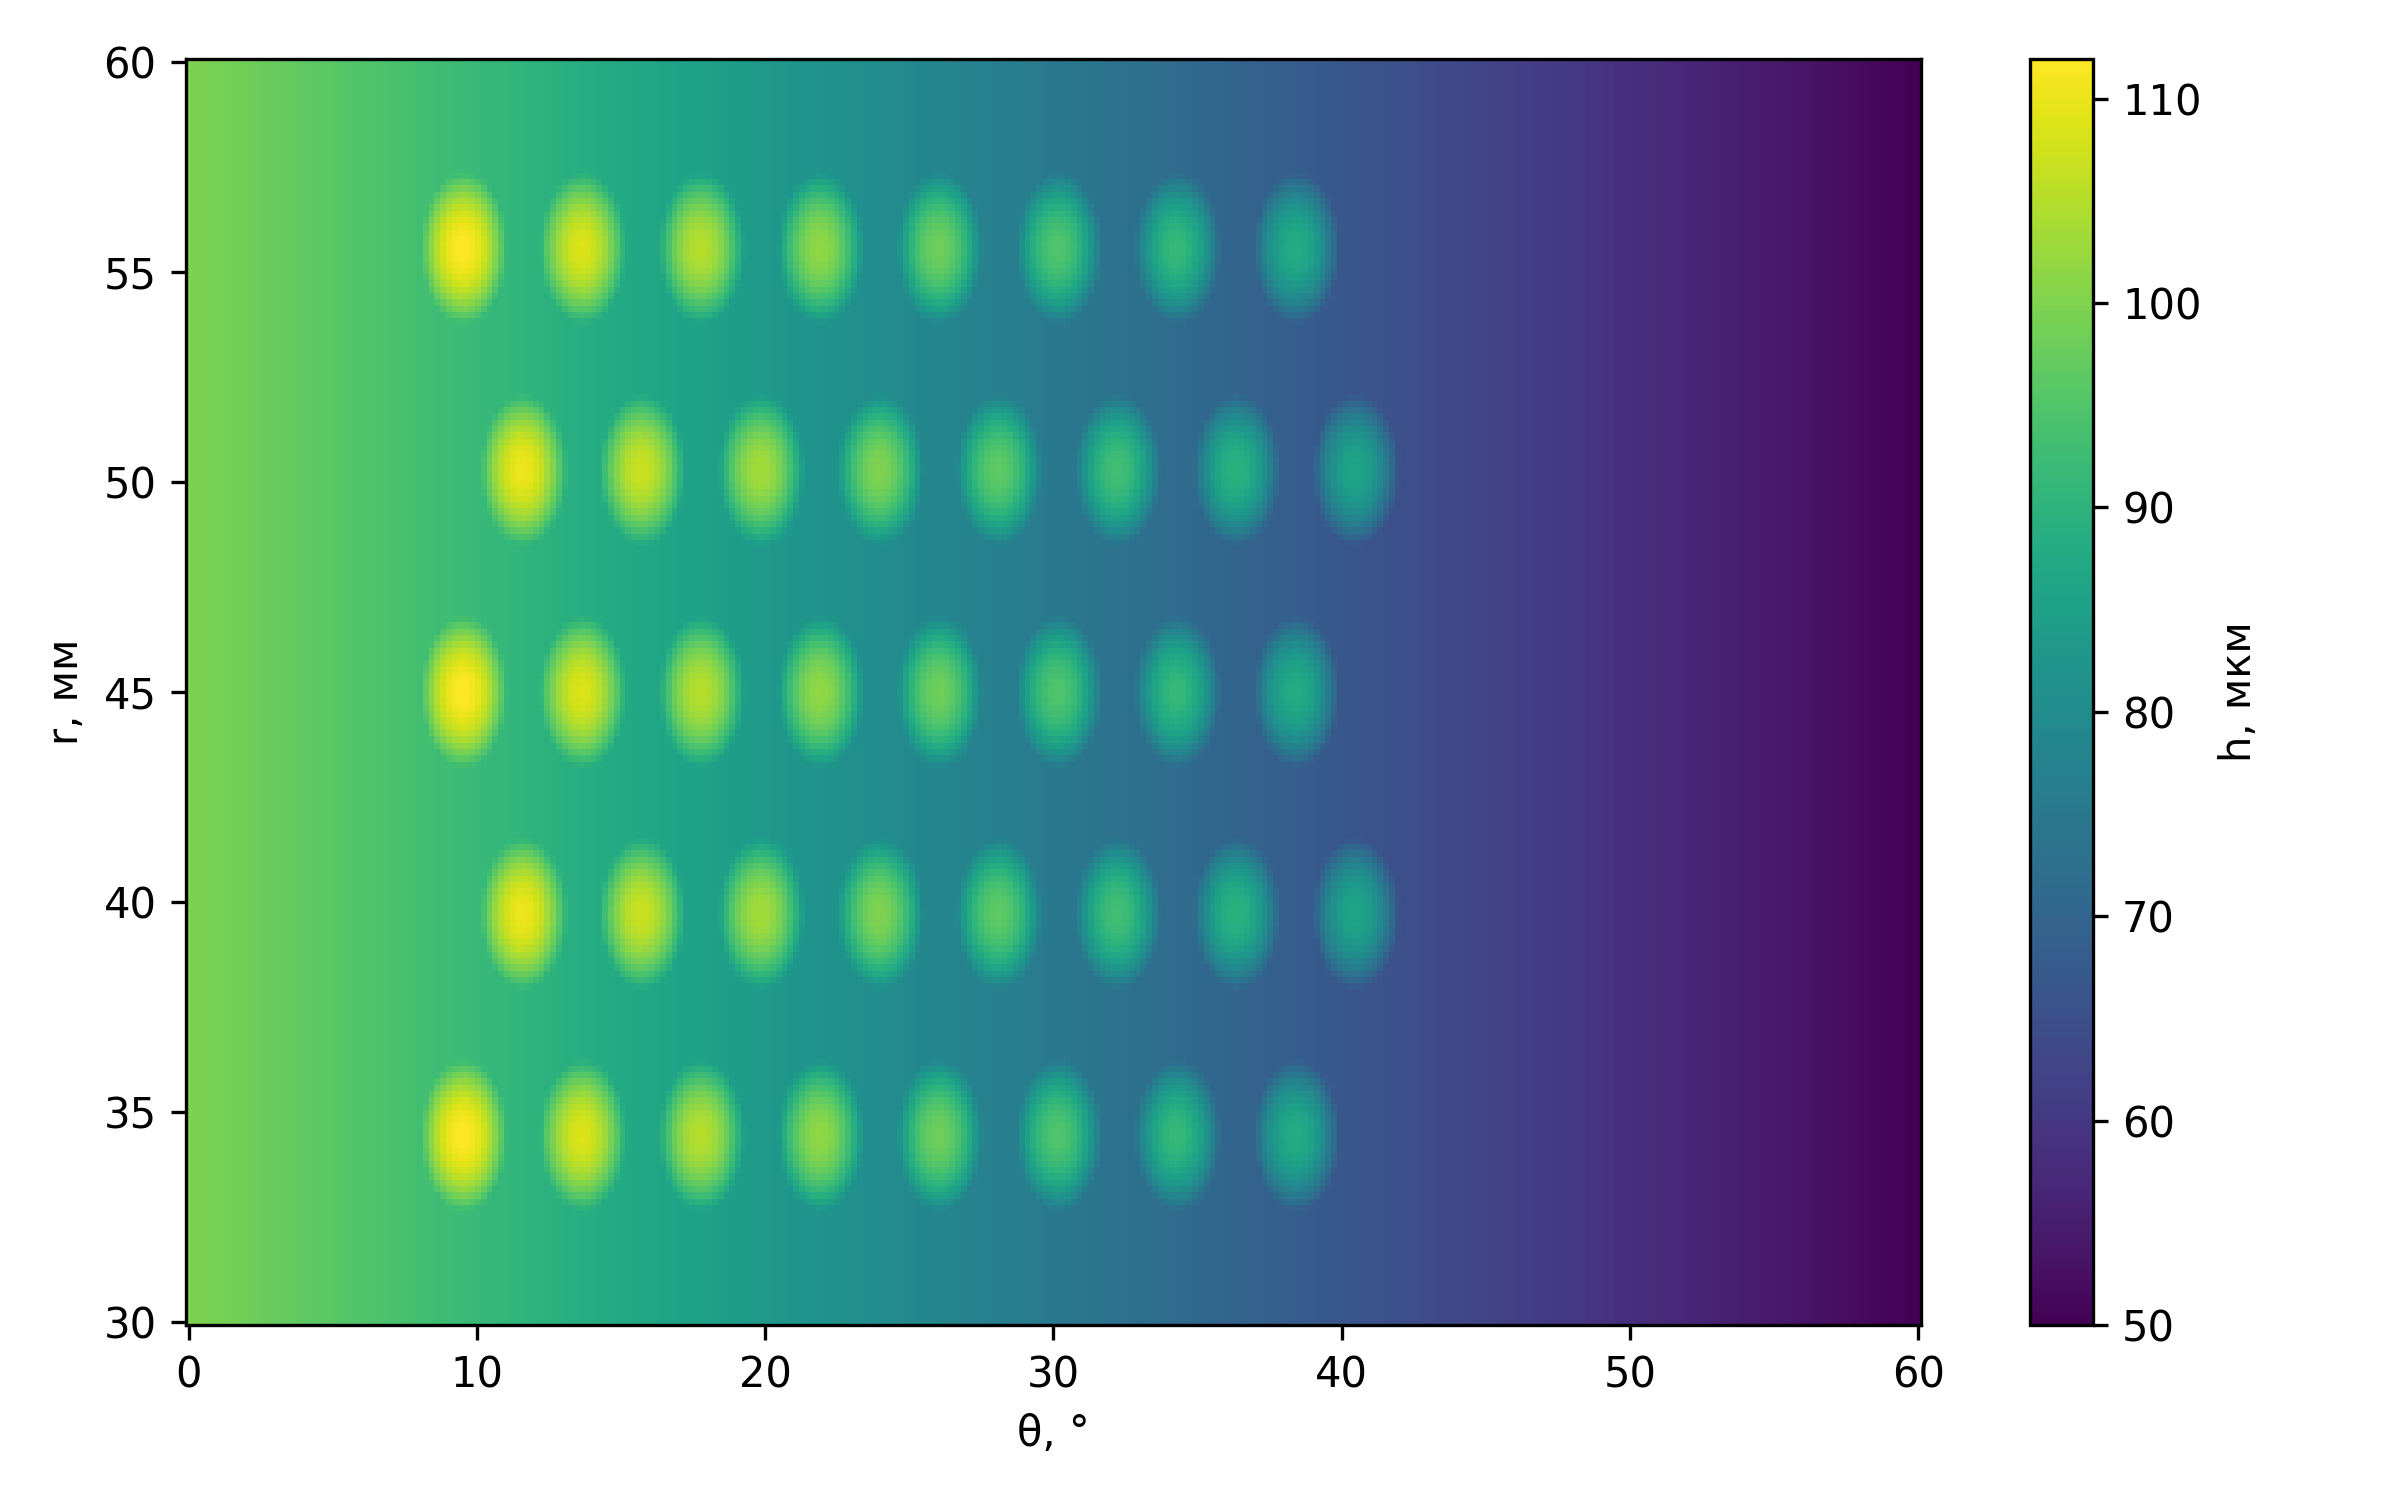
\includegraphics[width=\textwidth,height=0.9\textheight,keepaspectratio]{figures/ch07/fig_7_2.png}
\caption{Карта распределения зазора $h(r, \theta)$ в мкм
  для конфигурации~T2
  ($H_p = 0{,}40$, зона $0{,}1\beta$--$0{,}7\beta$) при $K = 2{,}0$.
  Светлые пятна~-- эллипсоидальные лунки.}
\label{fig:thrust_texture_map}
\end{figure}

\FloatBarrier


\section{Численная реализация расчёта}

Расчётная область дискретизируется равномерной сеткой
$200 \times 300$ узлов по~$r$ и~$\theta$. Уравнение
Рейнольдса~\eqref{eq:thrust_reynolds} аппроксимируется
центральными конечными разностями второго порядка точности.
Коэффициенты дивергентной формы вычисляются на полуузлах
$(i \pm 1/2,\; j \pm 1/2)$ с интерполяцией значений~$h$.

Полученная дискретная система решается итерационным
методом SOR (метод последовательной сверхрелаксации) с параметром
релаксации $\omega_{\mathrm{SOR}} = 1{,}5$. Критерий сходимости:
\begin{equation}
  \frac{\max |P_{\mathrm{new}} - P_{\mathrm{old}}|}
       {\max |P| + 10^{-10}} < 10^{-5}.
  \label{eq:thrust_convergence}
\end{equation}
Кавитация учитывается обнулением отрицательных давлений
на каждой итерации. Сходимость достигается за 2500--8000 итераций
в зависимости от~$K$ и конфигурации текстуры.


\section{Результаты при номинальном параметре клина}

При $K_{\mathrm{nom}} = 2{,}0$ проведён расчёт гладкого
подшипника и конфигураций T1, T2, T3. Результаты приведены
в таблице~\ref{tab:thrust_results}.

\begin{table}[!ht]
\centering
\caption{Характеристики упорного подшипника при $K_{\mathrm{nom}} = 2{,}0$}
\label{tab:thrust_results}
\begin{tabularx}{\textwidth}{|X|c|c|c|c|c|}
\hline
\multicolumn{1}{|c|}{\textbf{Вариант}}
  & $\boldsymbol{W}$, \textbf{кН}
  & $\boldsymbol{M_f}$, \textbf{Н$\cdot$м}
  & $\boldsymbol{f_T}$
  & $\boldsymbol{Q}$, \textbf{мл/с}
  & $\boldsymbol{p_{\max}}$, \textbf{МПа} \\
\hline
Гладкий & 1{,}82 & 1{,}6624 & 0{,}01953 & 26{,}595 & 0{,}510 \\
\hline
T1      & 1{,}84 & 1{,}6458 & 0{,}01912 & 27{,}007 & 0{,}536 \\
\hline
T2      & 1{,}85 & 1{,}6315 & 0{,}01889 & 27{,}324 & 0{,}552 \\
\hline
T3      & 1{,}79 & 1{,}6407 & 0{,}01963 & 26{,}406 & 0{,}523 \\
\hline
\end{tabularx}
\end{table}

\FloatBarrier

В рассматриваемой постановке минимальный зазор определяется
выходной кромкой колодки:
$h_{\min} = h_{\mathrm{out}} = 50$~мкм для всех вариантов
при фиксированной геометрии колодки, поэтому показатель
$G_{h_{\min}} = 1$ для всех конфигураций.

Нормированные показатели эффективности вычисляются аналогично
главам~5 и~6:
\begin{equation}
\begin{split}
  &G_W = \frac{W_{\mathrm{tex}}}{W_{\mathrm{smooth}}}, \quad
  G_{M_f} = \frac{M_{f,\mathrm{smooth}}}{M_{f,\mathrm{tex}}}, \\
  &G_{f_T} = \frac{f_{T,\mathrm{smooth}}}{f_{T,\mathrm{tex}}}, \quad
  G_Q = \frac{Q_{\mathrm{smooth}}}{Q_{\mathrm{tex}}}, \quad
  G_{p_{\max}} = \frac{p_{\max,\mathrm{smooth}}}{p_{\max,\mathrm{tex}}}.
\end{split}
  \label{eq:thrust_gains}
\end{equation}
Значение~$G > 1$ желательно для~$G_W$, $G_{M_f}$, $G_{f_T}$
(рост несущей способности, снижение момента трения и коэффициента
трения); для~$G_Q$ и~$G_{p_{\max}}$ значение~$G > 1$ означает
снижение расхода и пикового давления. Результаты сведены
в таблицу~\ref{tab:thrust_gains}.

\begin{table}[!ht]
\centering
\caption{Нормированные показатели эффективности
  при $K_{\mathrm{nom}} = 2{,}0$}
\label{tab:thrust_gains}
\begin{tabularx}{\textwidth}{|X|c|c|c|c|c|}
\hline
\multicolumn{1}{|c|}{\textbf{Вариант}}
  & $\boldsymbol{G_W}$
  & $\boldsymbol{G_{M_f}}$
  & $\boldsymbol{G_{f_T}}$
  & $\boldsymbol{G_Q}$
  & $\boldsymbol{G_{p_{\max}}}$ \\
\hline
T1 & 1{,}0107 & 1{,}0101 & 1{,}0209 & 0{,}9847 & 0{,}9517 \\
\hline
T2 & 1{,}0145 & 1{,}0189 & 1{,}0337 & 0{,}9733 & 0{,}9228 \\
\hline
T3 & 0{,}9816 & 1{,}0132 & 0{,}9946 & 1{,}0071 & 0{,}9738 \\
\hline
\end{tabularx}
\end{table}

\FloatBarrier

Конфигурации T1 и~T2, расположенные во входной и средней части
клина, обеспечивают умеренный рост несущей способности:
$G_W = 1{,}0107$ и $1{,}0145$. Коэффициент трения снижается:
$G_{f_T} = 1{,}0209$ и $1{,}0337$ ($G_{f_T} > 1$ означает снижение
$f_T$). Прирост~$W$ сопровождается увеличением расхода~$Q$
и максимального давления~$p_{\max}$
($G_Q < 1$, $G_{p_{\max}} < 1$).

Конфигурация~T3, нанесённая в средней и выходной части клина,
снижает несущую способность ($G_W = 0{,}9816 < 1$) и не улучшает
коэффициент трения ($G_{f_T} = 0{,}9946 < 1$). Это подтверждает
гипотезу: текстура в зоне убывания давления неэффективна.

Таким образом, текстурирование во входной и средней зоне (T1,~T2)
улучшает несущую способность и трение, однако увеличивает утечки
и пиковое давление. Наилучший баланс демонстрирует
конфигурация~T2: $G_W = 1{,}0145$, $G_{f_T} = 1{,}0337$,
$G_{p_{\max}} = 0{,}9228$.

Нормированные показатели наглядно сопоставлены на
рисунке~\ref{fig:thrust_gains}.

\begin{figure}[!ht]
\centering
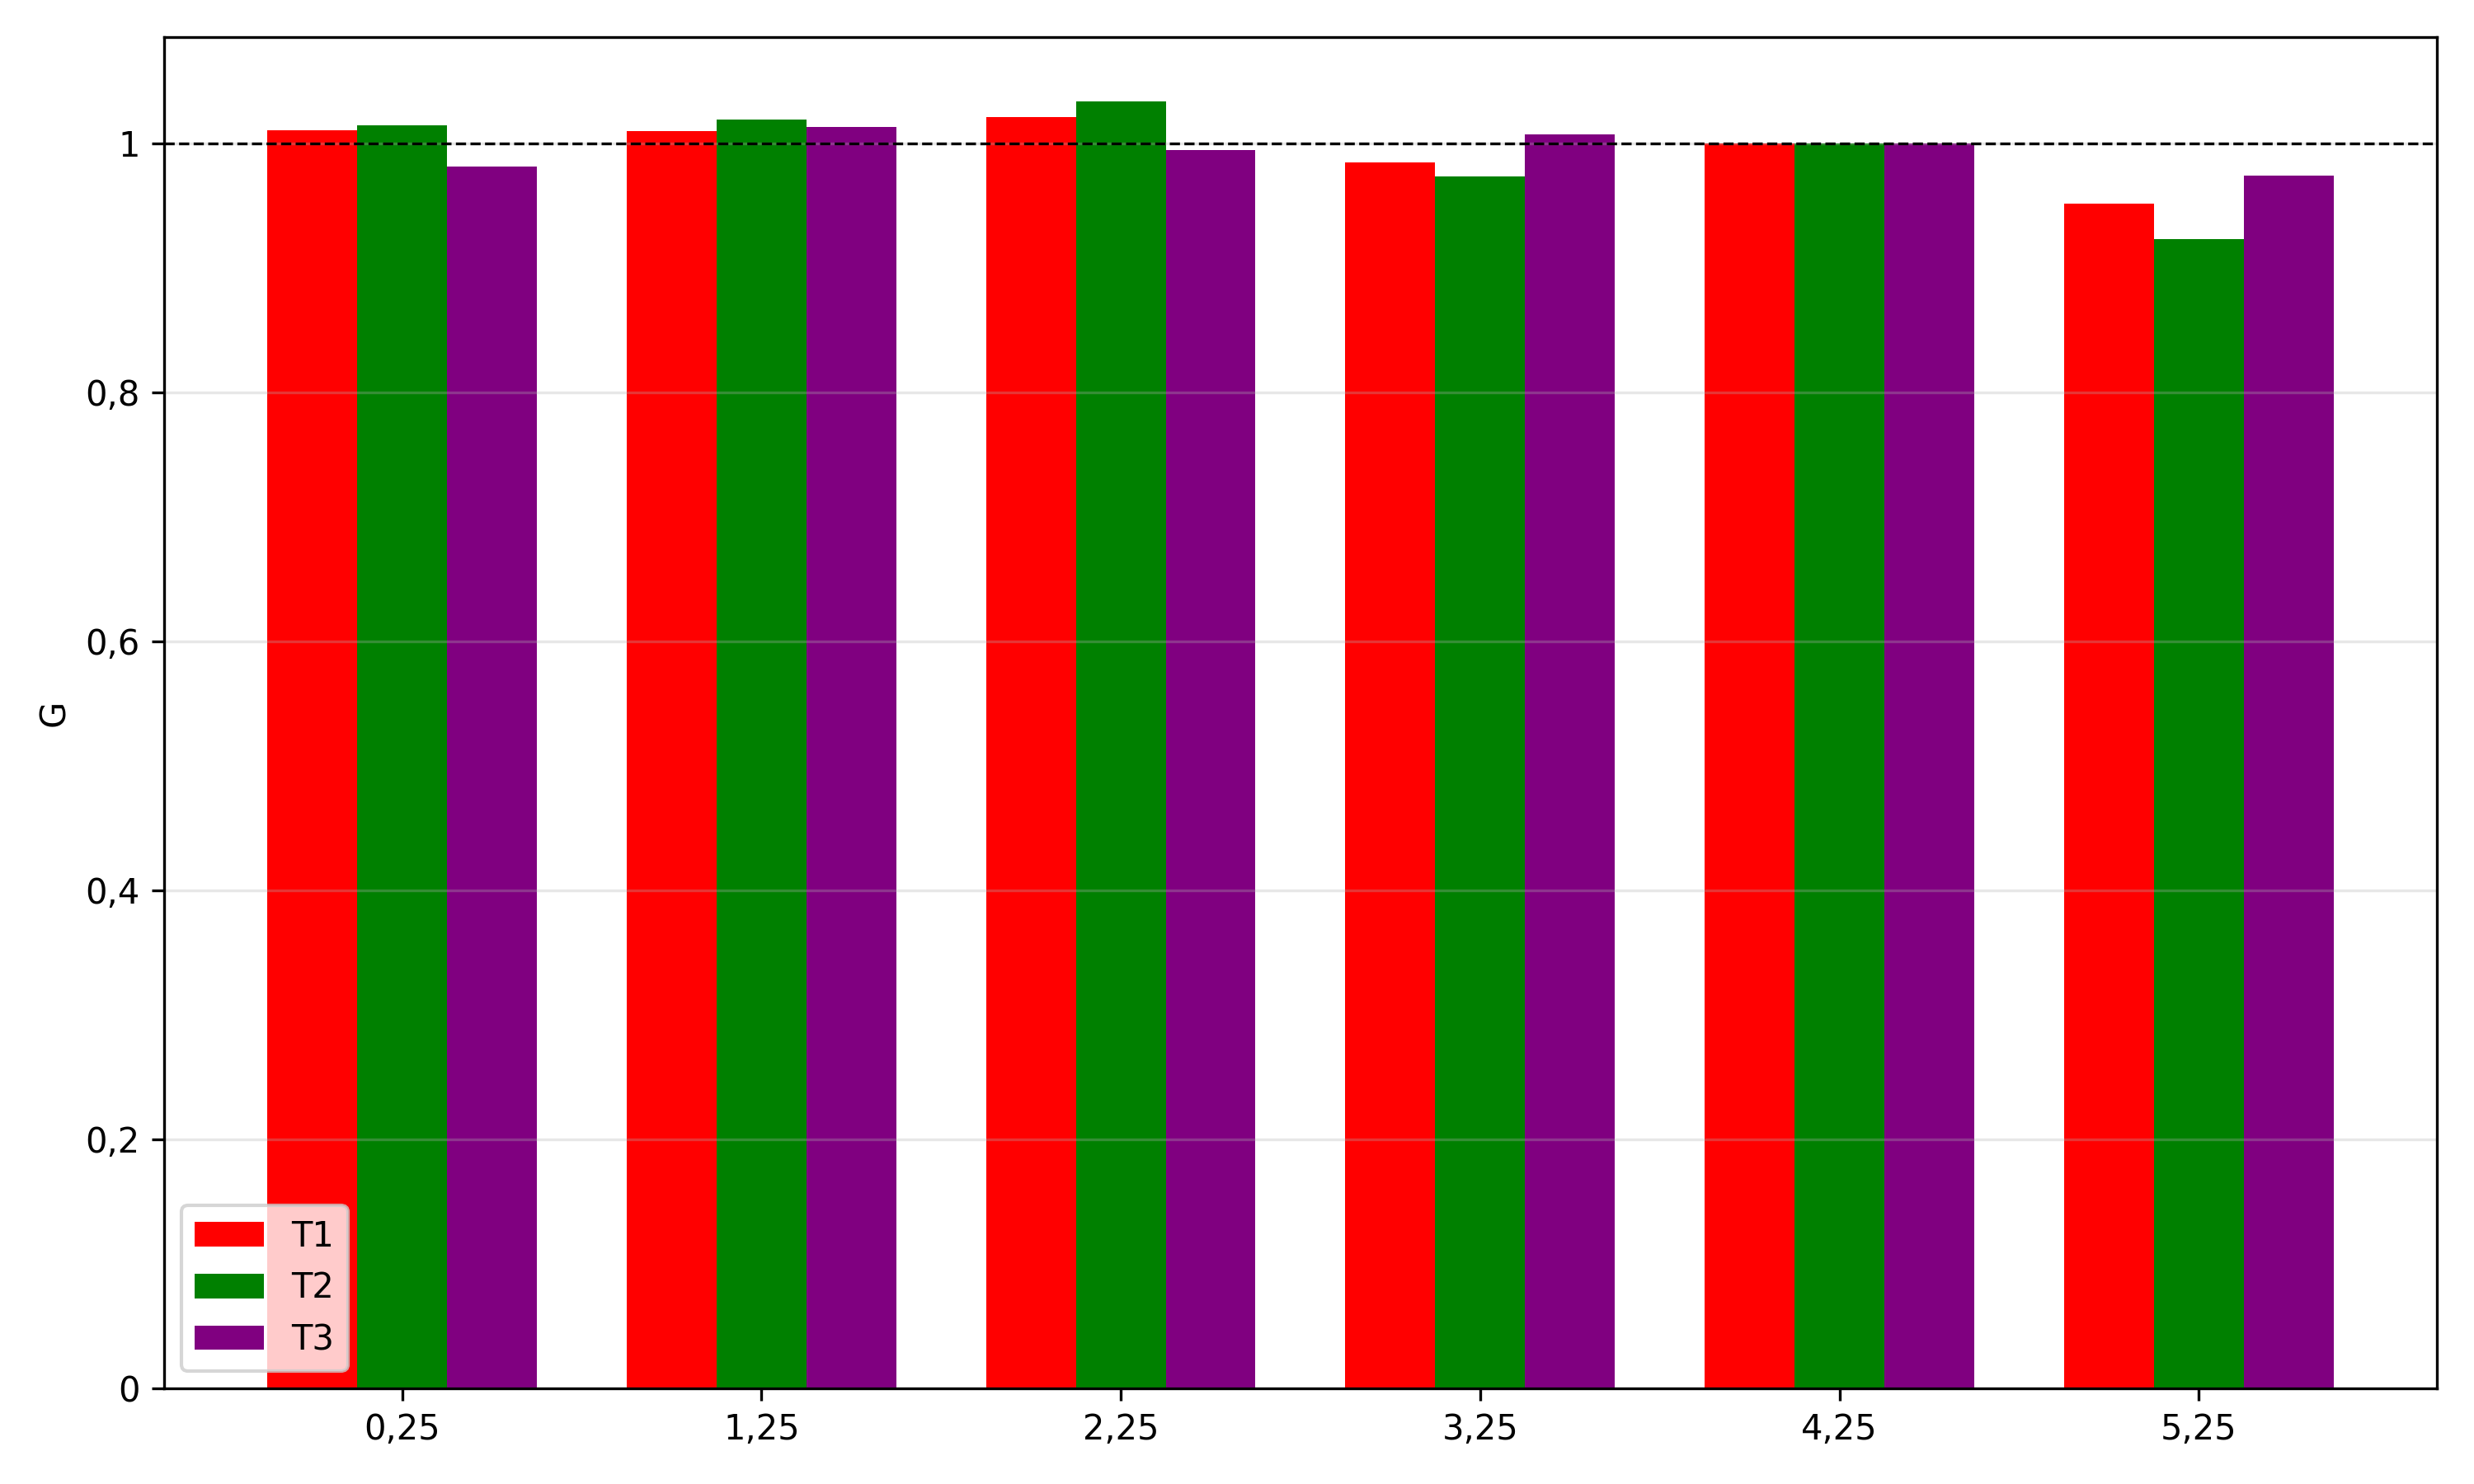
\includegraphics[width=\textwidth,height=0.9\textheight,keepaspectratio]{figures/ch07/fig_7_3.png}
\caption{Нормированные показатели эффективности $G_W$, $G_{M_f}$,
  $G_{f_T}$, $G_Q$, $G_{p_{\max}}$ для конфигураций T1, T2, T3
  при $K_{\mathrm{nom}} = 2{,}0$. Пунктирная горизонталь $G = 1$~--
  уровень гладкого подшипника.}
\label{fig:thrust_gains}
\end{figure}

\FloatBarrier


\section{Влияние параметра клина на рабочие характеристики}

Параметрический расчёт выполнен для
$K \in \{1{,}5;\; 2{,}0;\; 2{,}5;\; 3{,}0;\; 3{,}5;\; 4{,}0\}$.

\textit{Несущая сила.}
Несущая сила~$W$ имеет максимум при $K \approx 2{,}5$ для всех
вариантов (рисунок~\ref{fig:thrust_W_vs_K})~-- классическая
особенность клинового подшипника: при малых~$K$ клин слаб,
при больших~$K$ зазор~$h_{\mathrm{in}}$ слишком велик и давление
падает. Конфигурация~T2 превышает гладкий вариант по всему
диапазону~$K$. Конфигурация~T3 уступает гладкому при всех~$K$.

\begin{figure}[!ht]
\centering
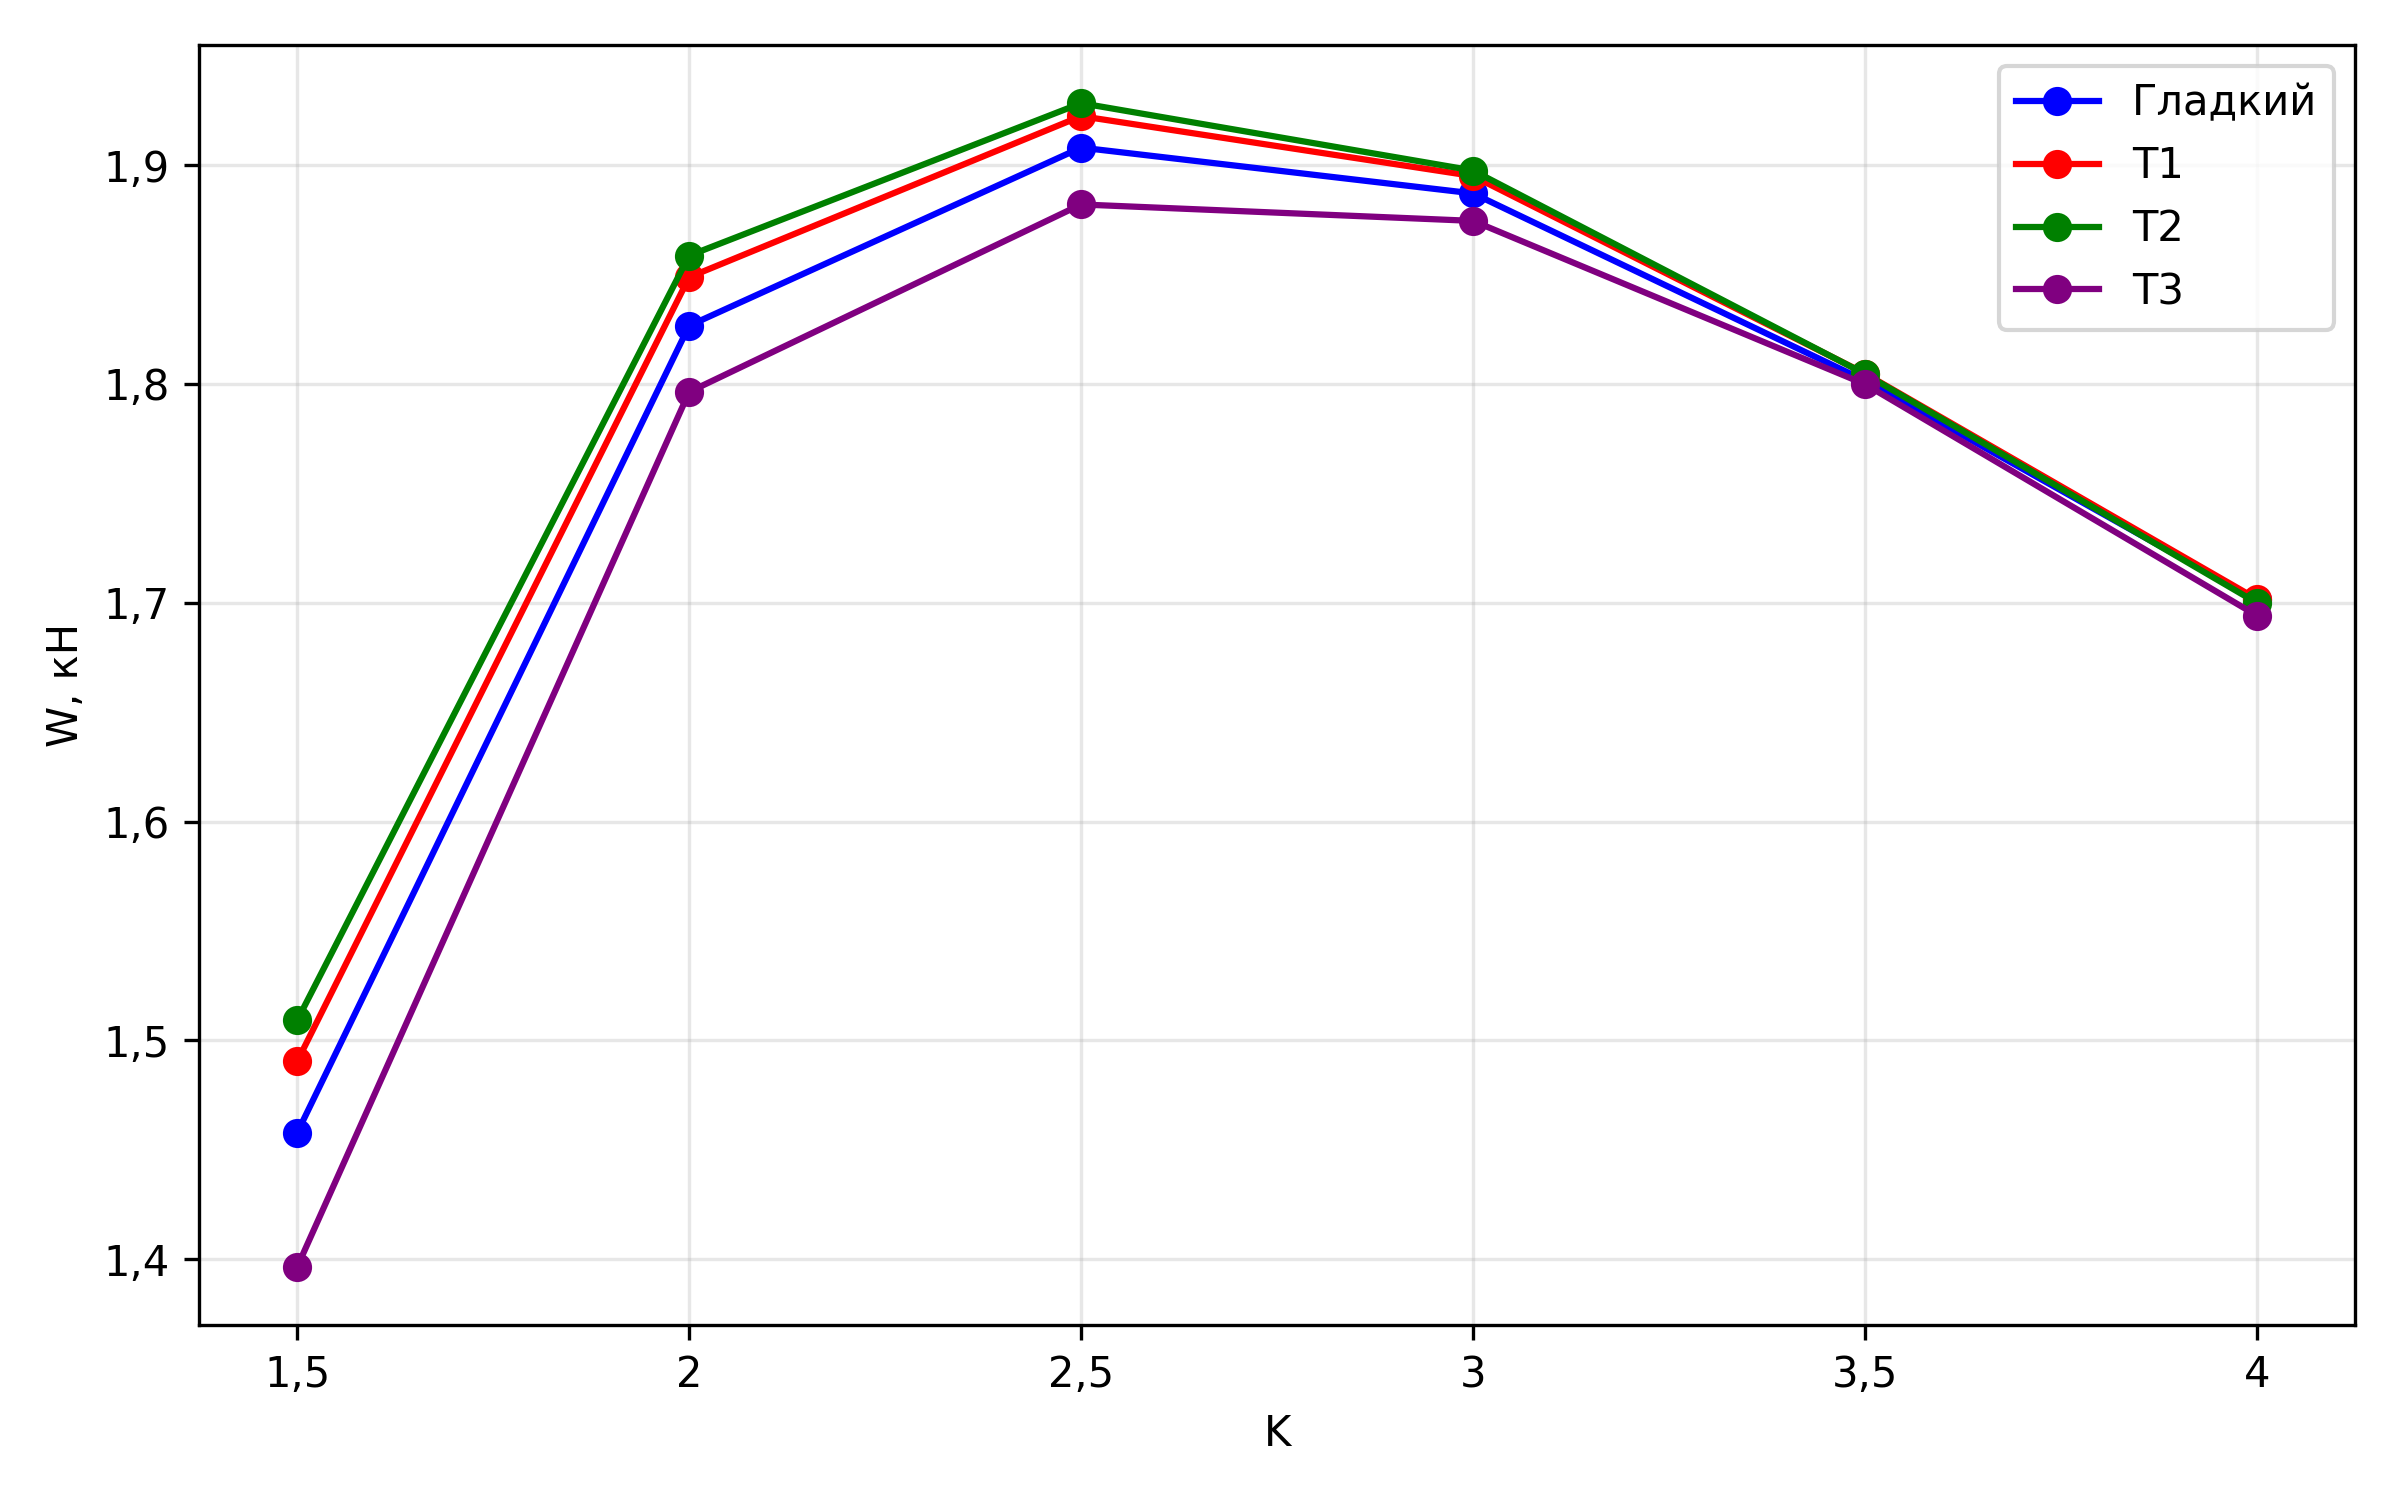
\includegraphics[width=\textwidth,height=0.9\textheight,keepaspectratio]{figures/ch07/fig_7_4.png}
\caption{Зависимость несущей силы $W$ от параметра клина $K$
  для гладкого подшипника и конфигураций T1, T2, T3.}
\label{fig:thrust_W_vs_K}
\end{figure}

\FloatBarrier

\textit{Коэффициент трения.}
Коэффициент трения~$f_T$ монотонно убывает с ростом~$K$
(рисунок~\ref{fig:thrust_fT_vs_K}). Конфигурация~T2 имеет
наименьший~$f_T$ при всех~$K$; конфигурация~T3 близка к гладкому
варианту или незначительно хуже.

\begin{figure}[!ht]
\centering
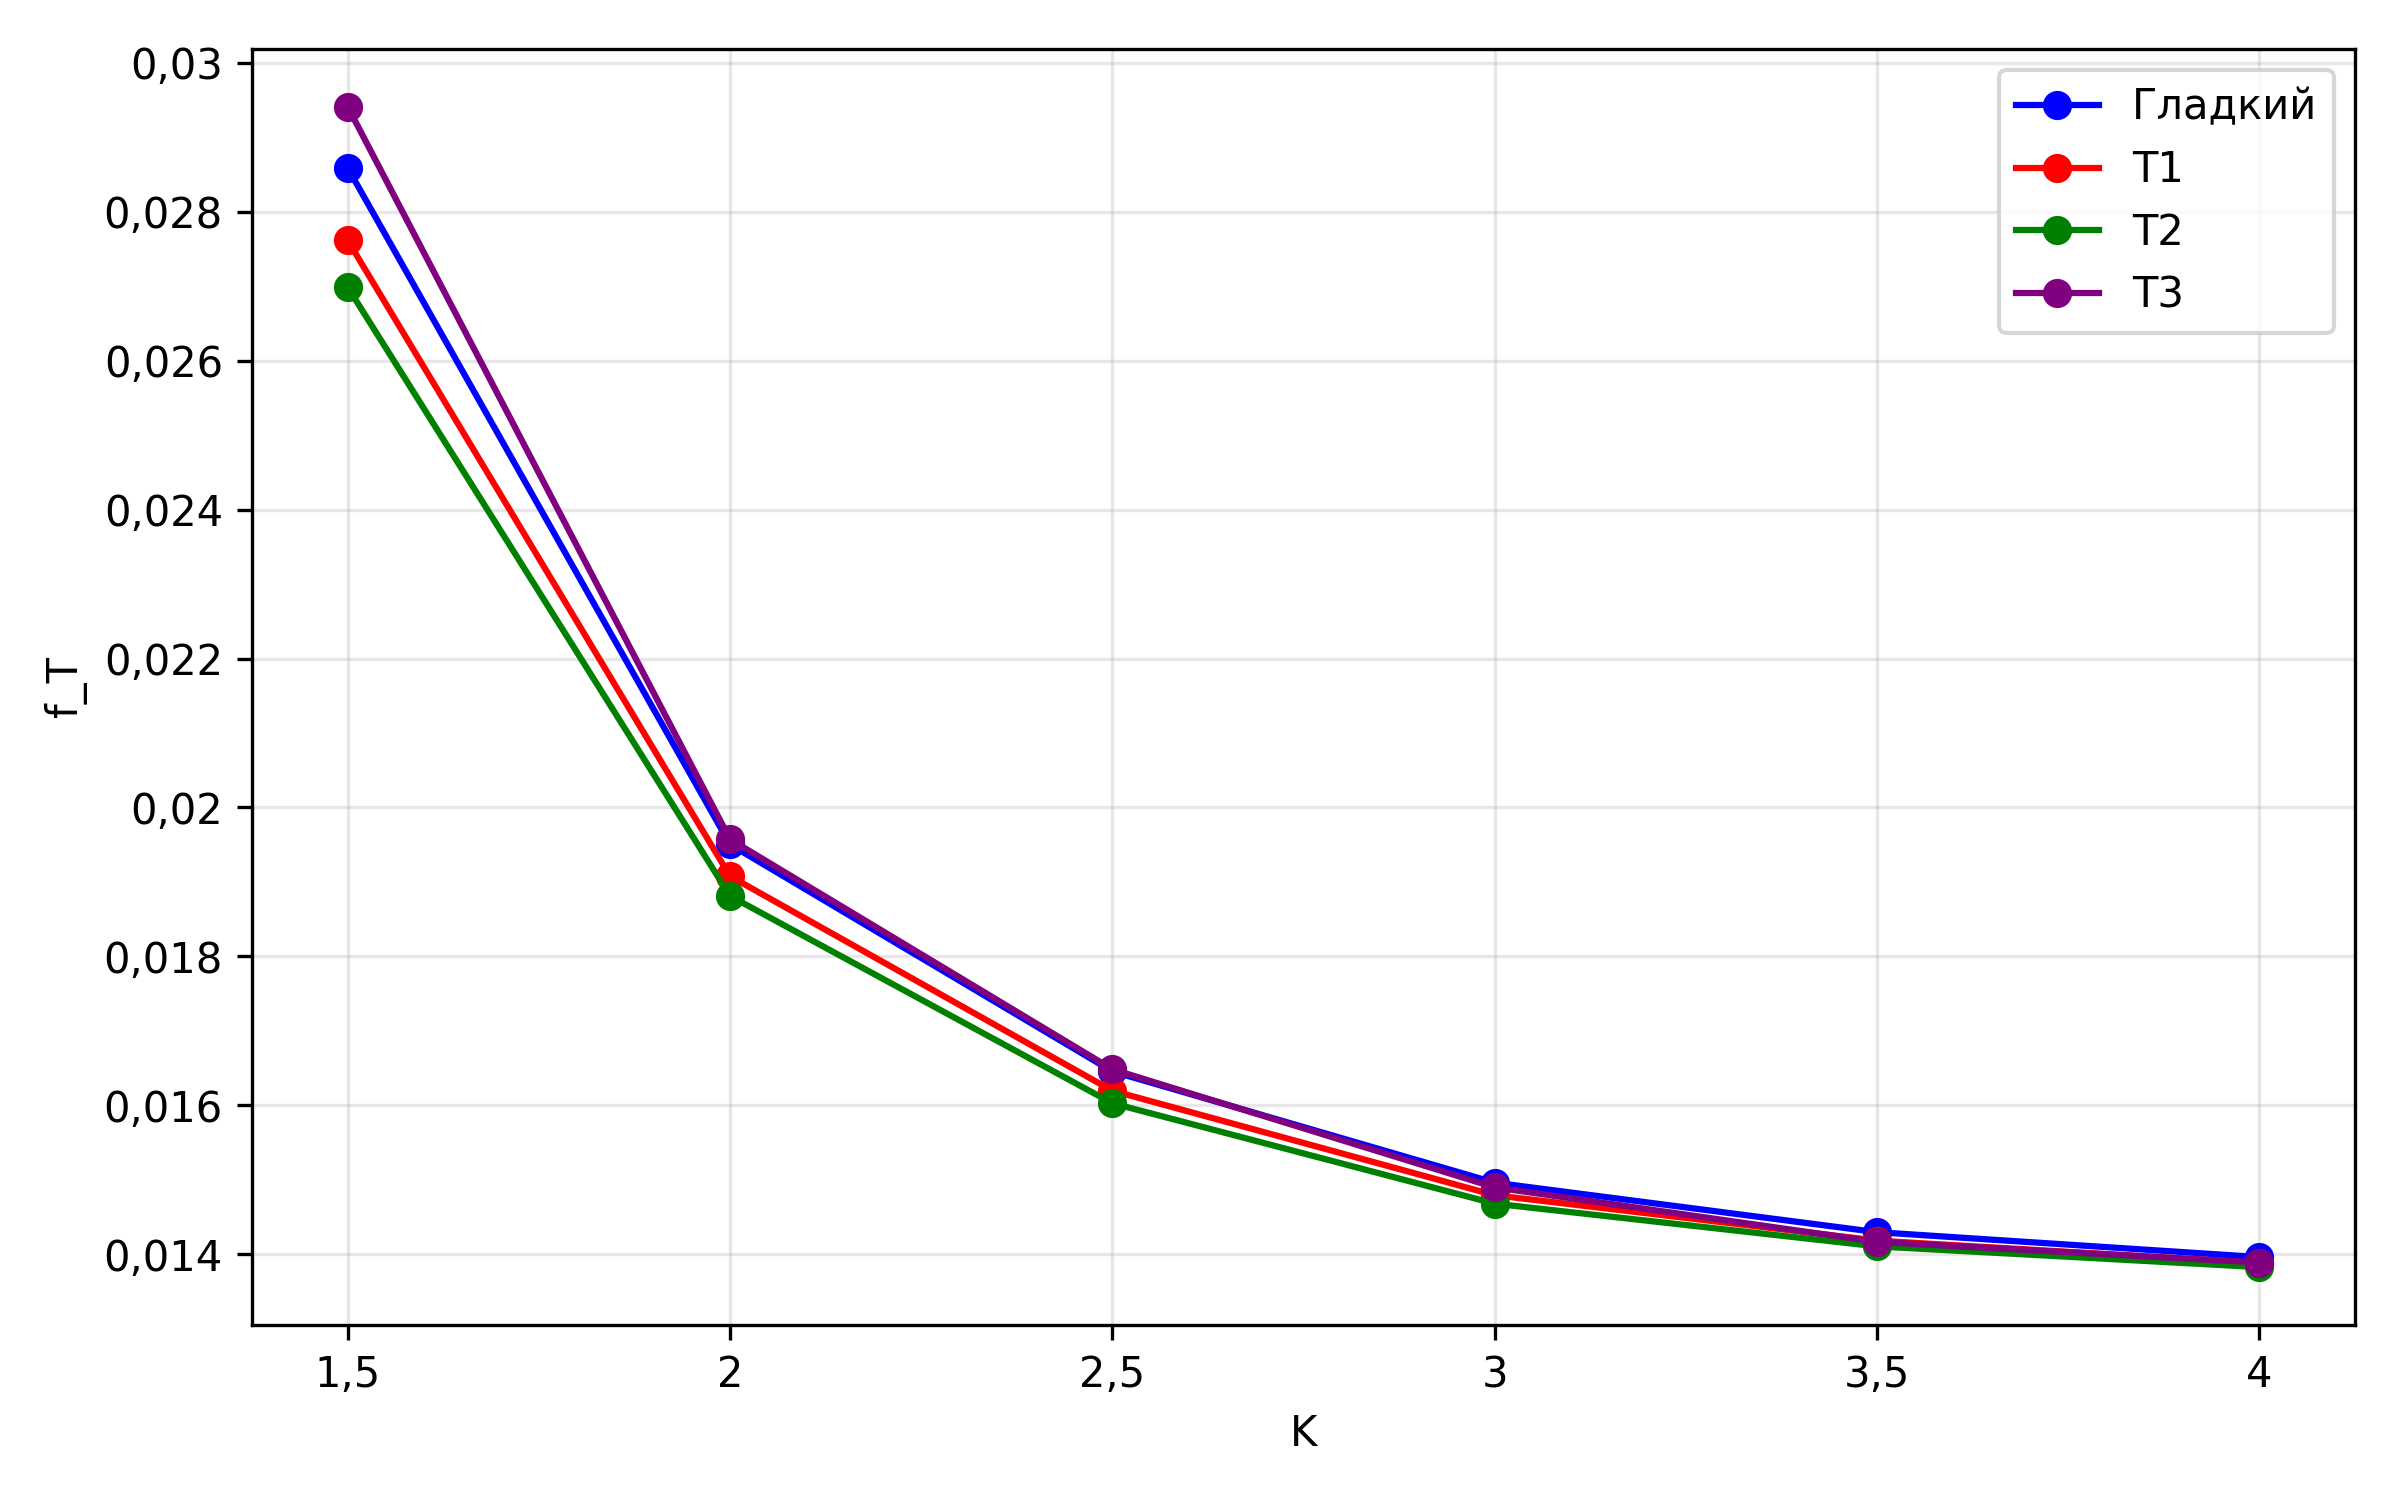
\includegraphics[width=\textwidth,height=0.9\textheight,keepaspectratio]{figures/ch07/fig_7_5.png}
\caption{Зависимость коэффициента трения $f_T$ от параметра
  клина $K$.}
\label{fig:thrust_fT_vs_K}
\end{figure}

\FloatBarrier

\textit{Расход смазочного материала.}
Расход~$Q$ монотонно растёт с~$K$
(рисунок~\ref{fig:thrust_Q_vs_K}). Различия между вариантами
невелики ($\leq 5\,\%$); конфигурация~T2 имеет несколько больший
расход вследствие увеличенного объёма лунок.

\begin{figure}[!ht]
\centering
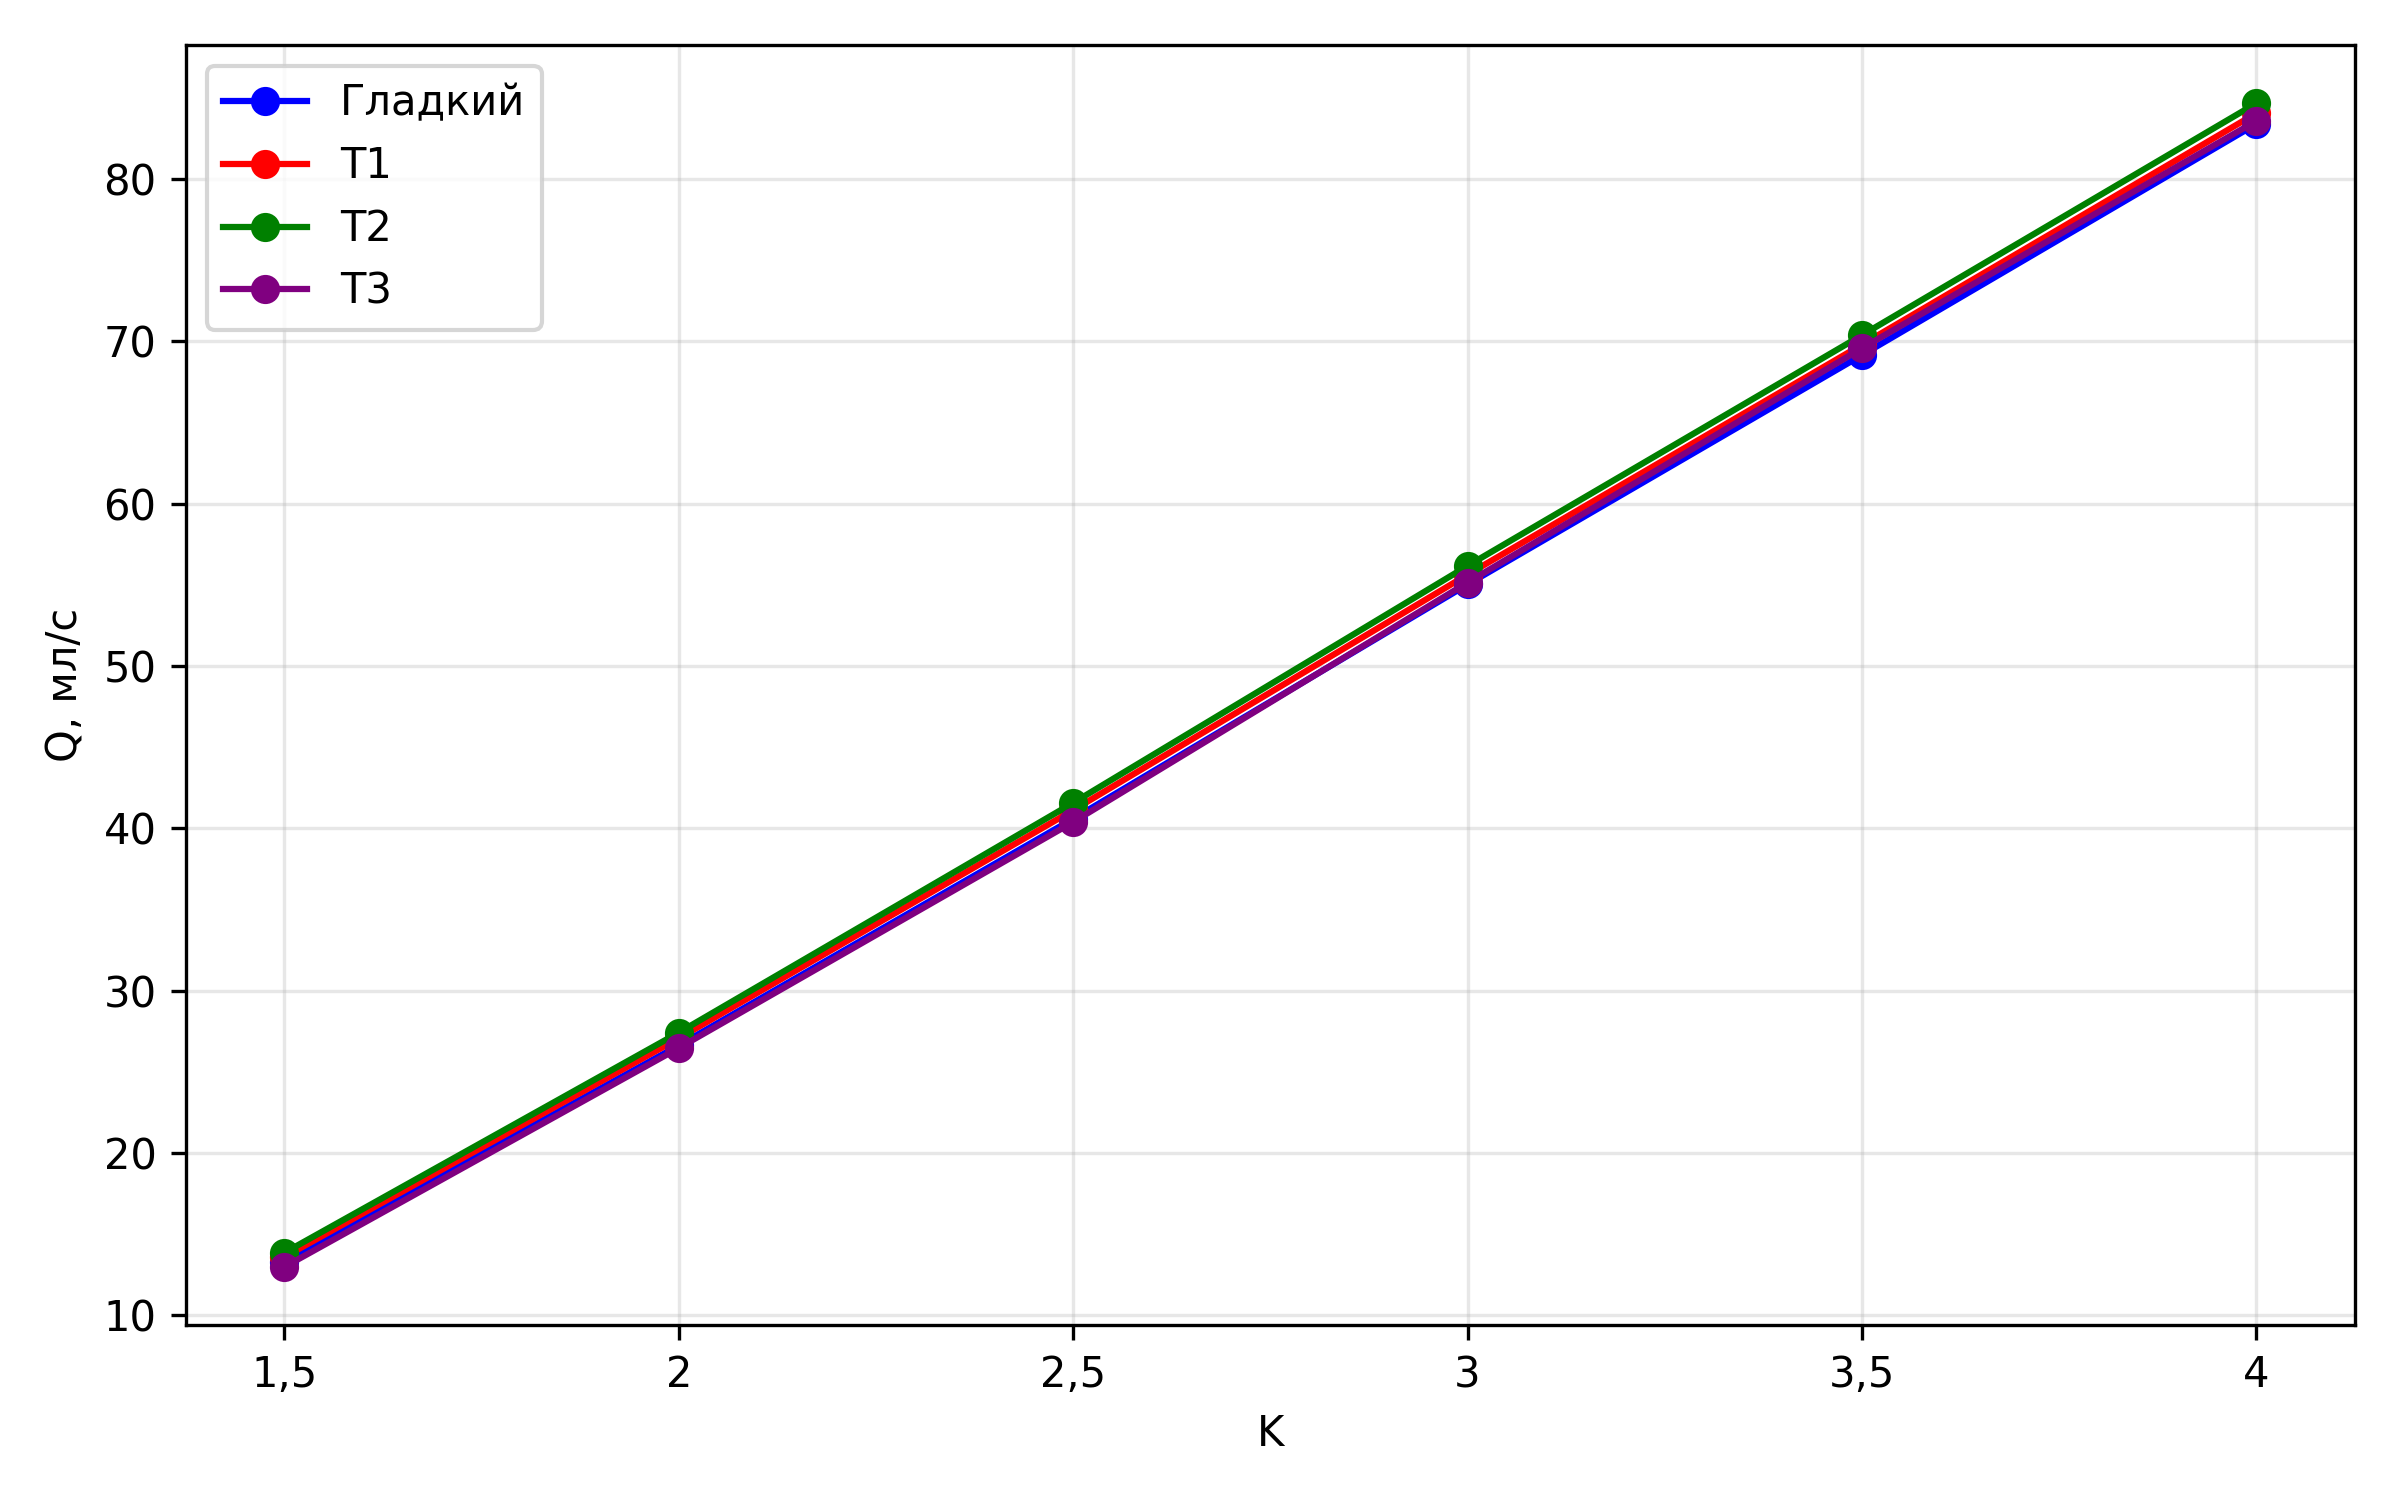
\includegraphics[width=\textwidth,height=0.9\textheight,keepaspectratio]{figures/ch07/fig_7_6.png}
\caption{Зависимость расхода смазки $Q$ от параметра клина $K$.}
\label{fig:thrust_Q_vs_K}
\end{figure}

\FloatBarrier

\textit{Максимальное давление.}
Максимальное давление~$p_{\max}$ растёт с~$K$ и достигает
насыщения при $K \approx 3$--$4$
(рисунок~\ref{fig:thrust_pmax_vs_K}). Конфигурации~T2 и~T1
демонстрируют более высокое~$p_{\max}$ по сравнению с гладким
вариантом; конфигурация~T3~-- ниже при малых~$K$ и выше
при больших~$K$.

\begin{figure}[!ht]
\centering
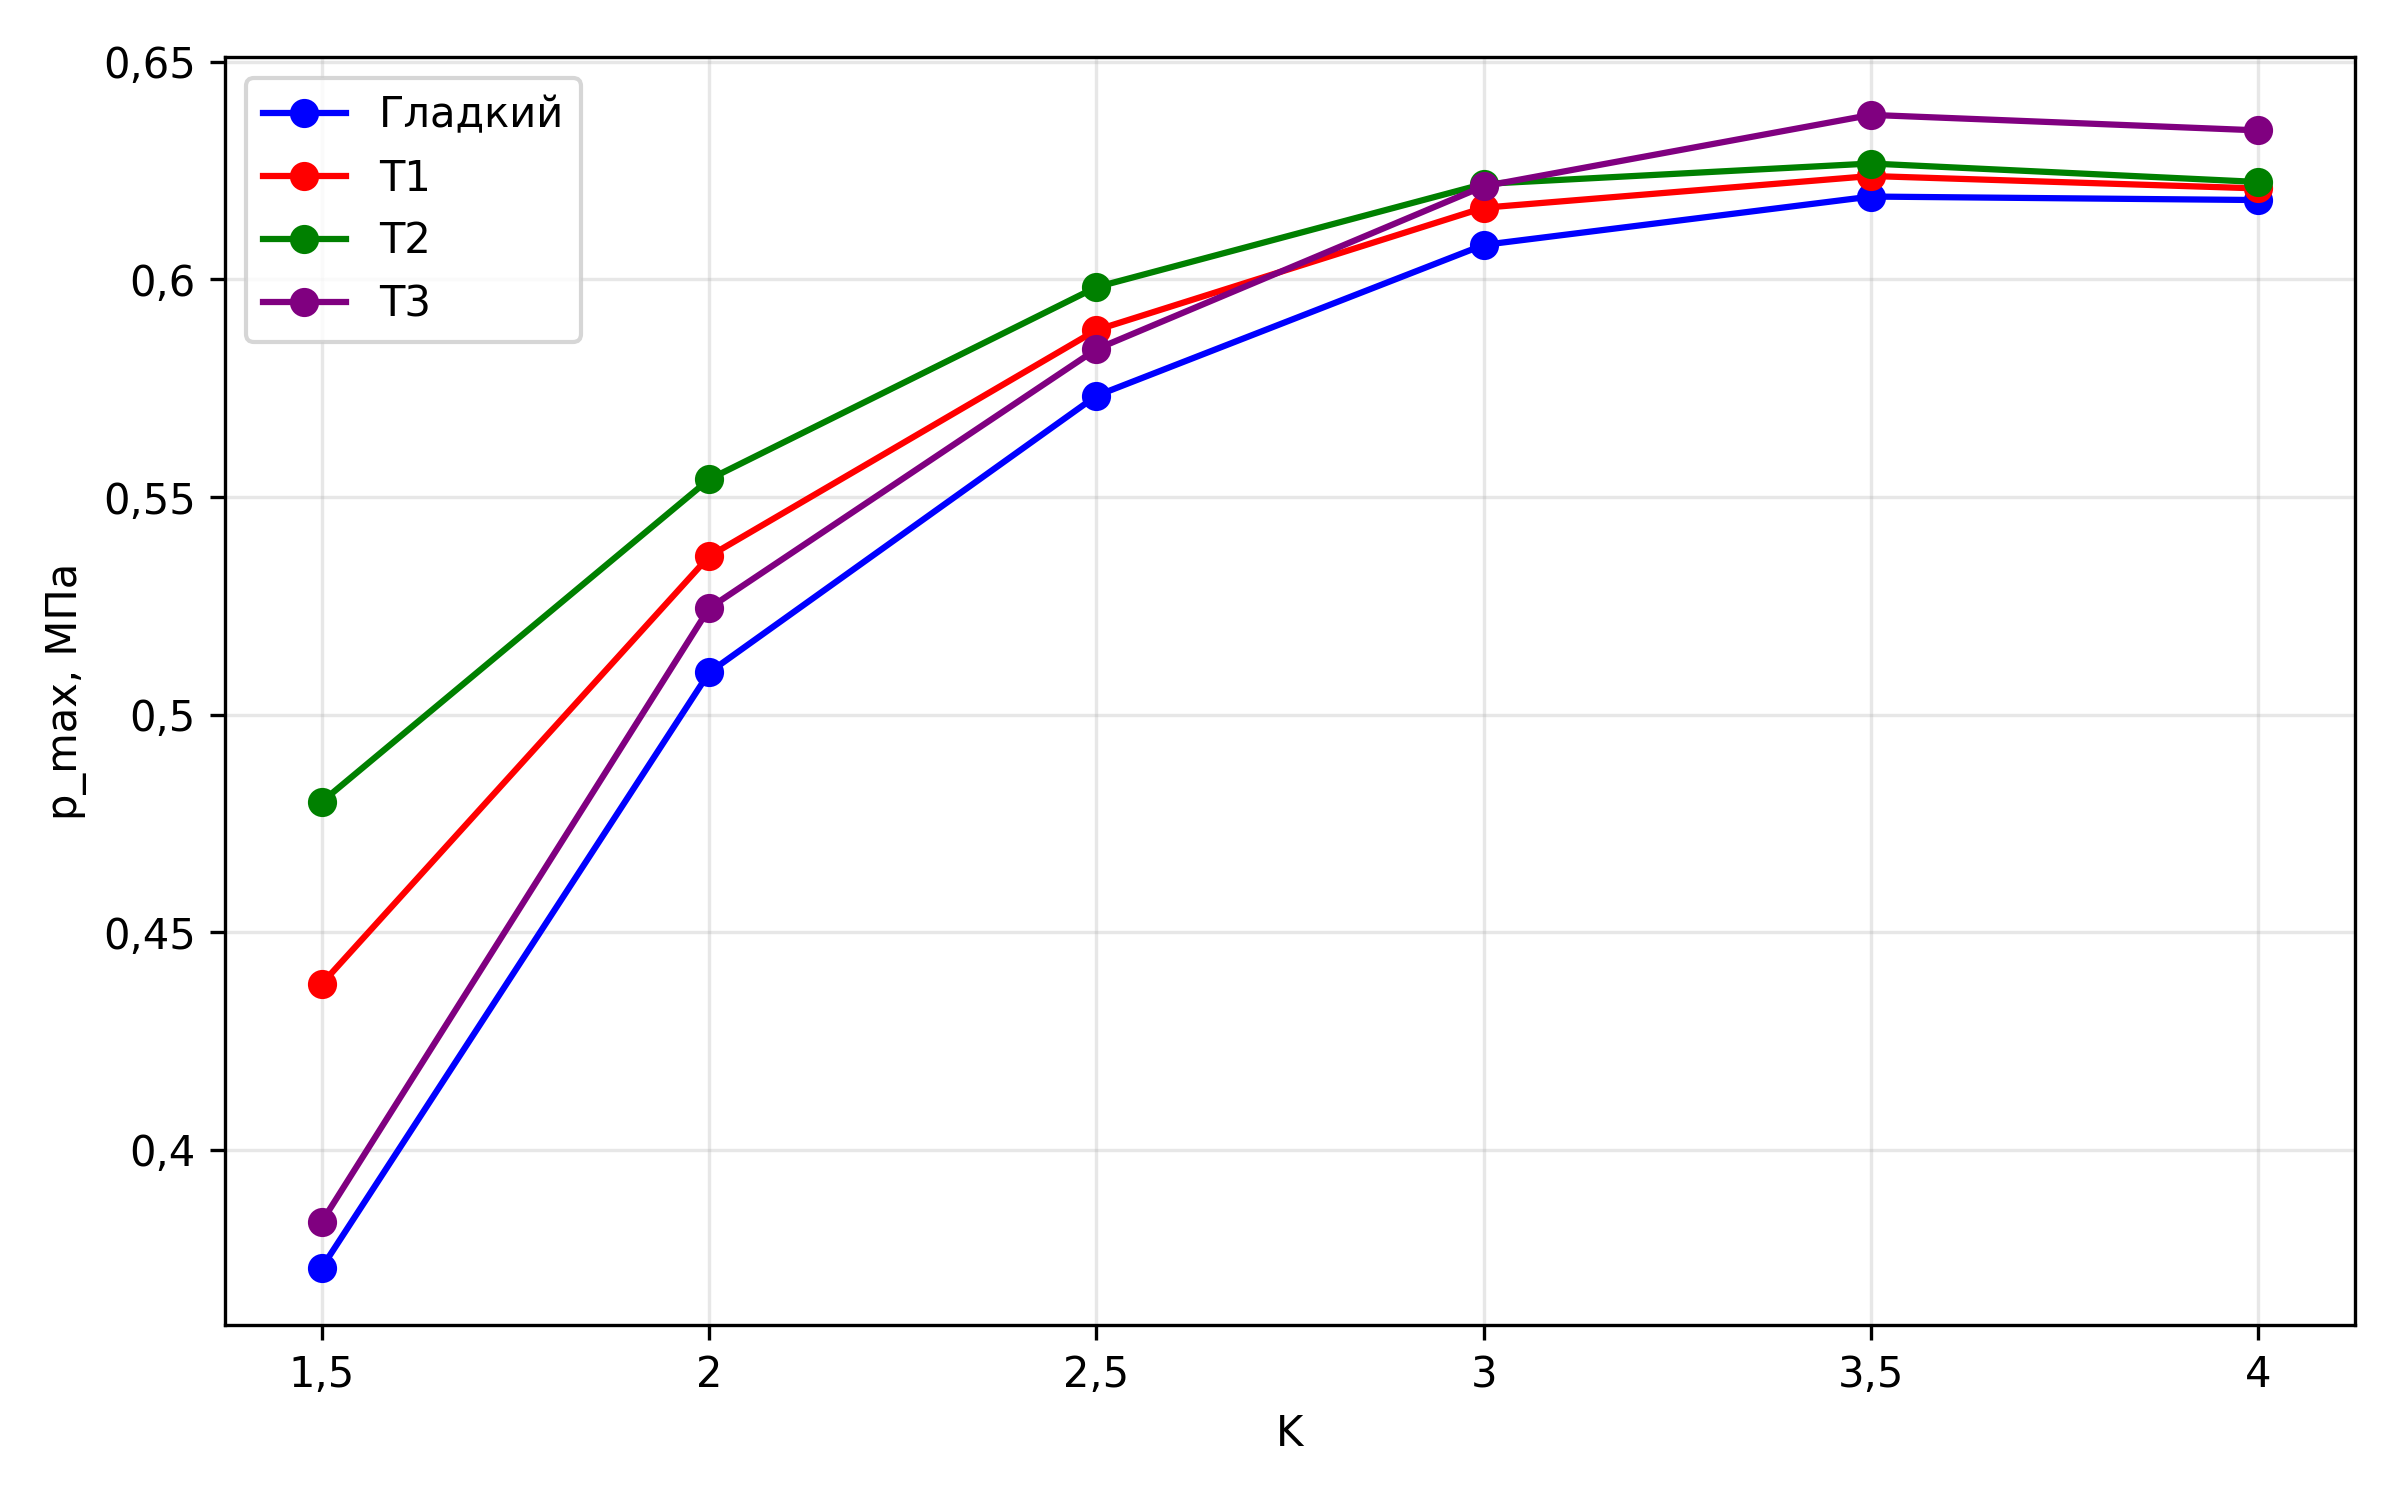
\includegraphics[width=\textwidth,height=0.9\textheight,keepaspectratio]{figures/ch07/fig_7_7.png}
\caption{Зависимость максимального давления $p_{\max}$ от параметра
  клина $K$.}
\label{fig:thrust_pmax_vs_K}
\end{figure}

\FloatBarrier

\textit{Минимальный зазор.}
В рассматриваемой постановке минимальный зазор определяется
выходной кромкой колодки:
$h_{\min} = h_{\mathrm{out}} = 50$~мкм для всех вариантов
и значений~$K$. Зависимость~$h_{\min}(K)$ не рассматривается.

\FloatBarrier


\section{Анализ распределения давления и обсуждение результатов}

\textit{Гладкий подшипник.}
Для гладкого подшипника поле давления $p(r, \theta)$ при
$K = 2{,}0$ имеет сглаженное распределение по радиусу
и единственный максимум в центральной части сектора
(рис.~\ref{fig:thrust_P3D_smooth}).
В рассматриваемой постановке при $K = 2{,}0$ во внутренней части
расчётной области не наблюдается выраженной области с нулевым
давлением; нулевые значения реализуются главным образом на
граничных кромках в соответствии с условиями~\eqref{eq:thrust_bc}.

\begin{figure}[!ht]
\centering
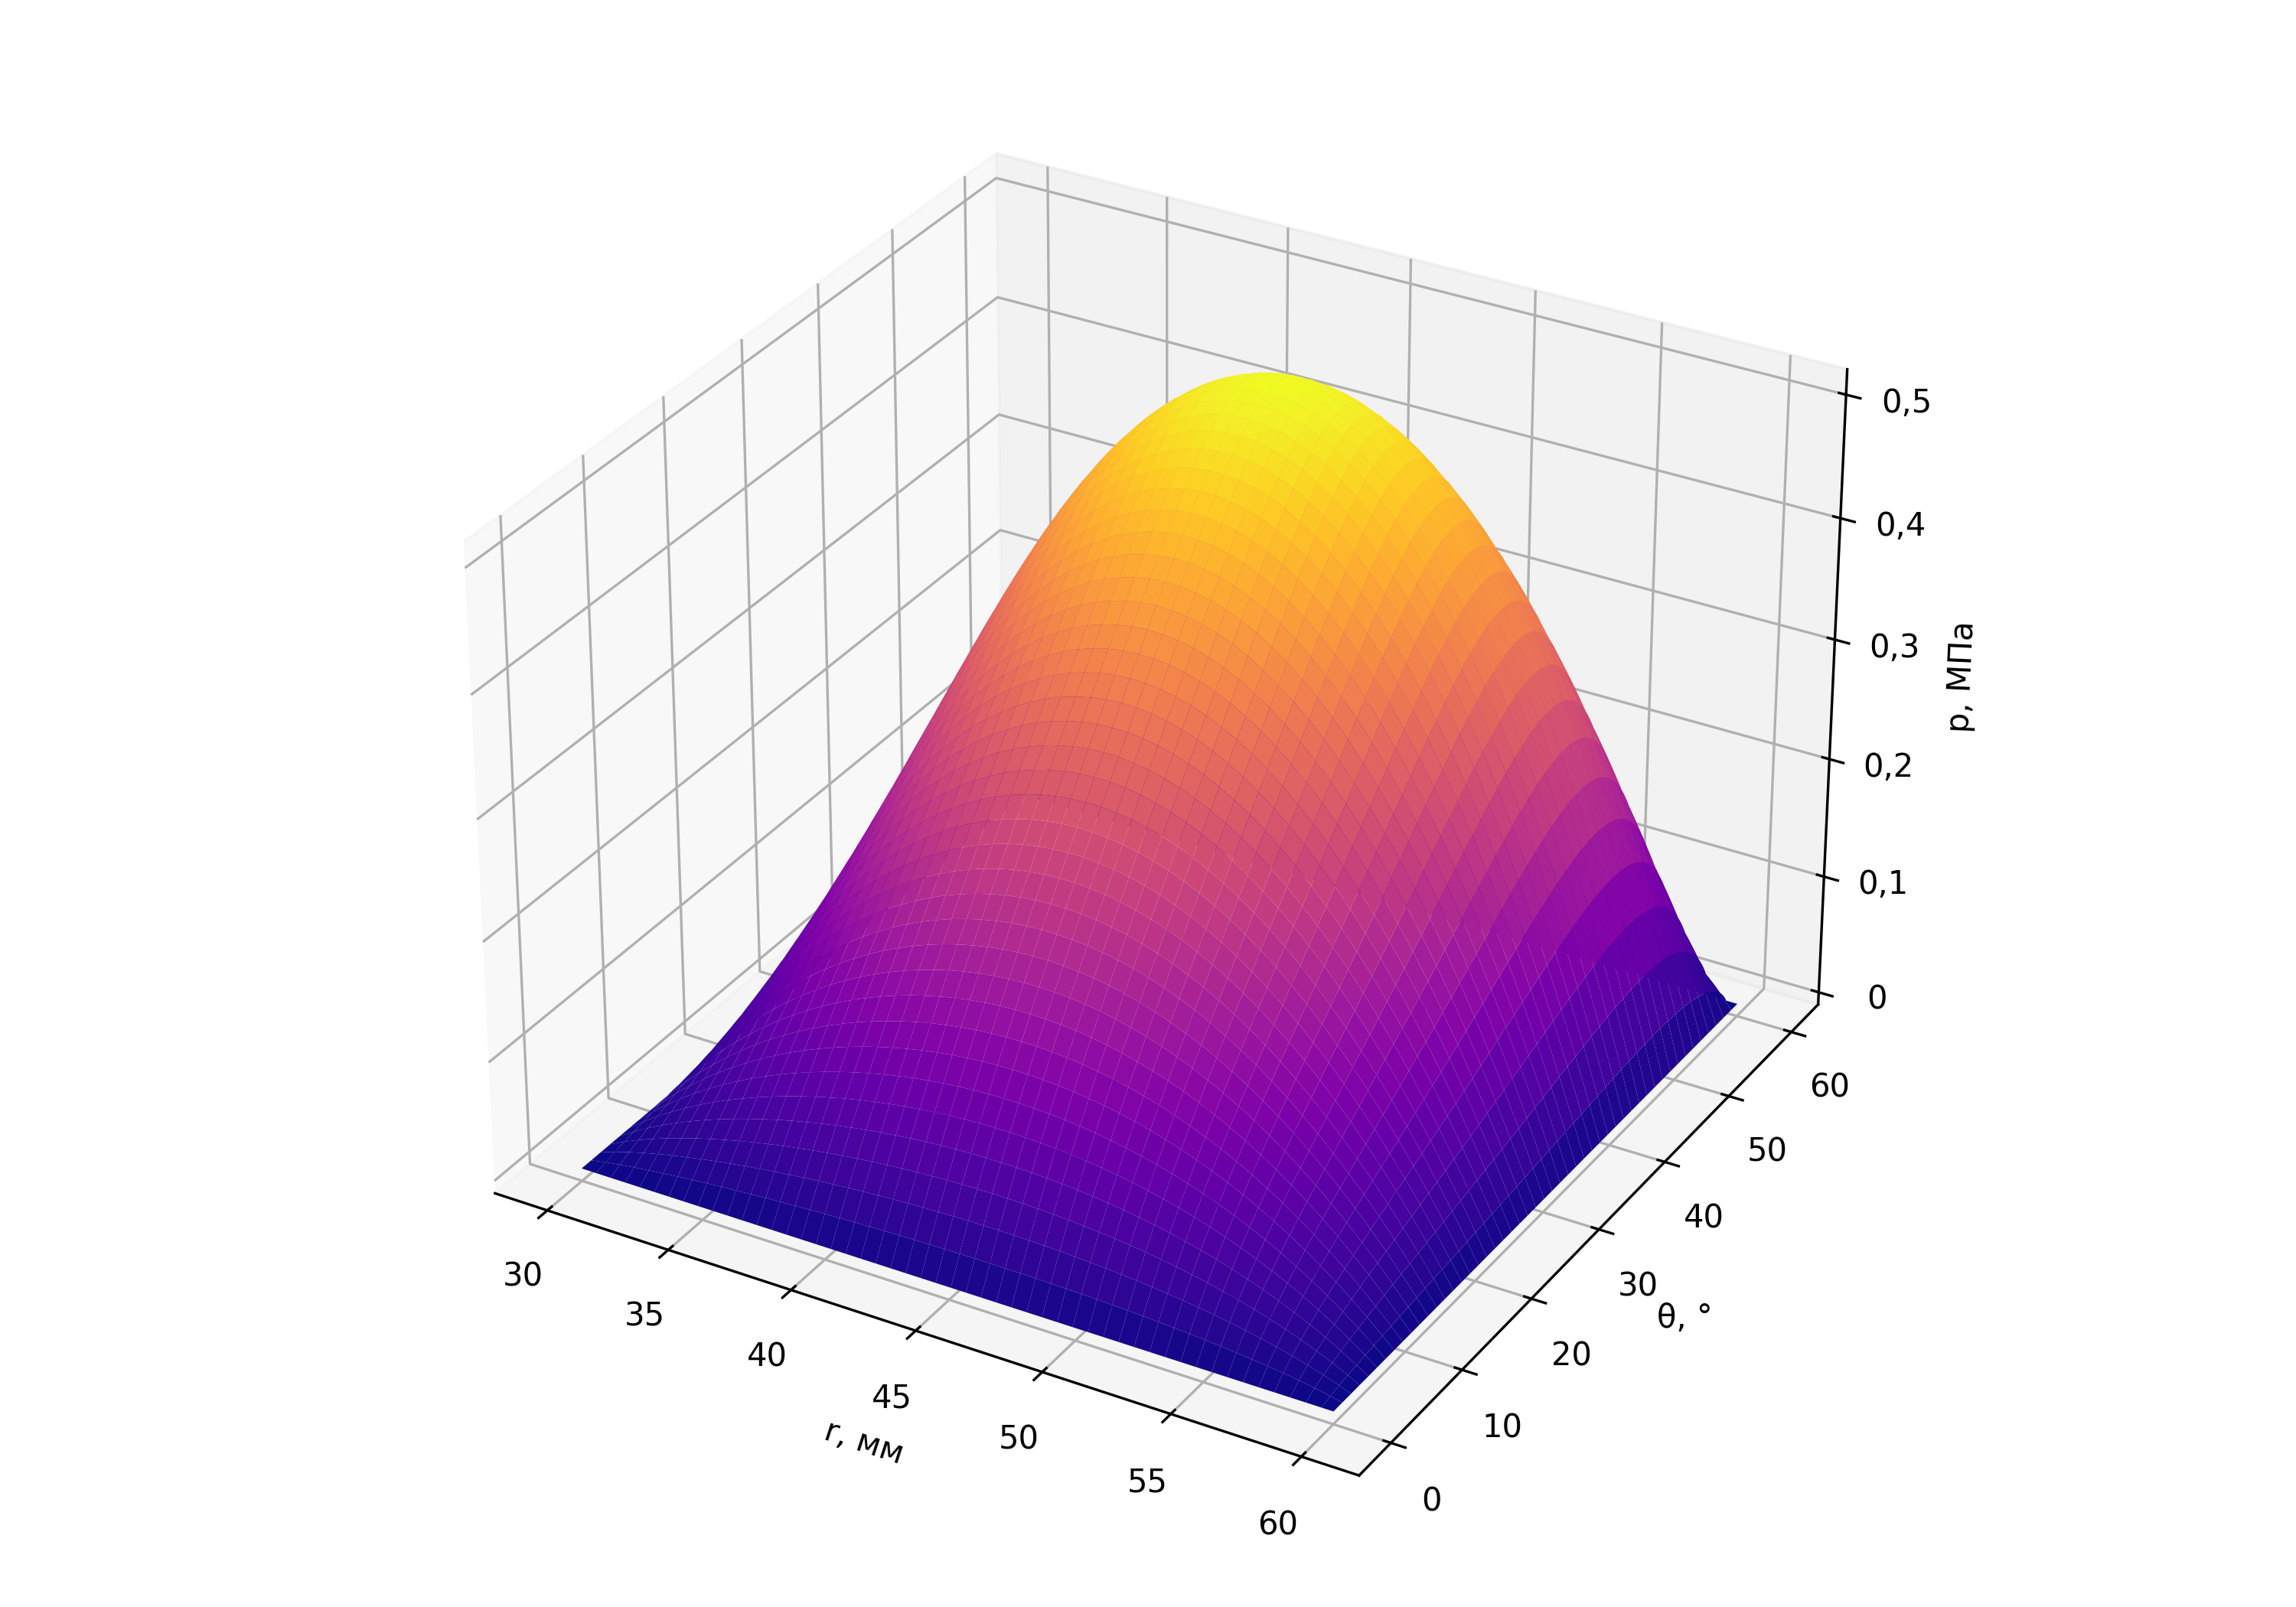
\includegraphics[width=\textwidth,height=0.9\textheight,keepaspectratio]{figures/ch07/fig_7_8.png}
\caption{Поле давления $p(r, \theta)$ гладкого подшипника
  при $K_{\mathrm{nom}} = 2{,}0$.}
\label{fig:thrust_P3D_smooth}
\end{figure}

\FloatBarrier

\textit{Конфигурация~T2.}
Текстурирование поверхности по конфигурации~T2 приводит к появлению
локальных пиков давления над лунками во входной и средней части
сектора (<<рябь>> на поверхности $p(r, \theta)$, рис.~\ref{fig:thrust_P3D_T2}). Интегральная
несущая сила возрастает вследствие дополнительных гидродинамических
клиньев, формируемых передними стенками лунок. В выходной части
сектора ($\theta > 0{,}7\beta$), свободной от текстуры, профиль
давления близок к гладкому случаю.

\begin{figure}[!ht]
\centering
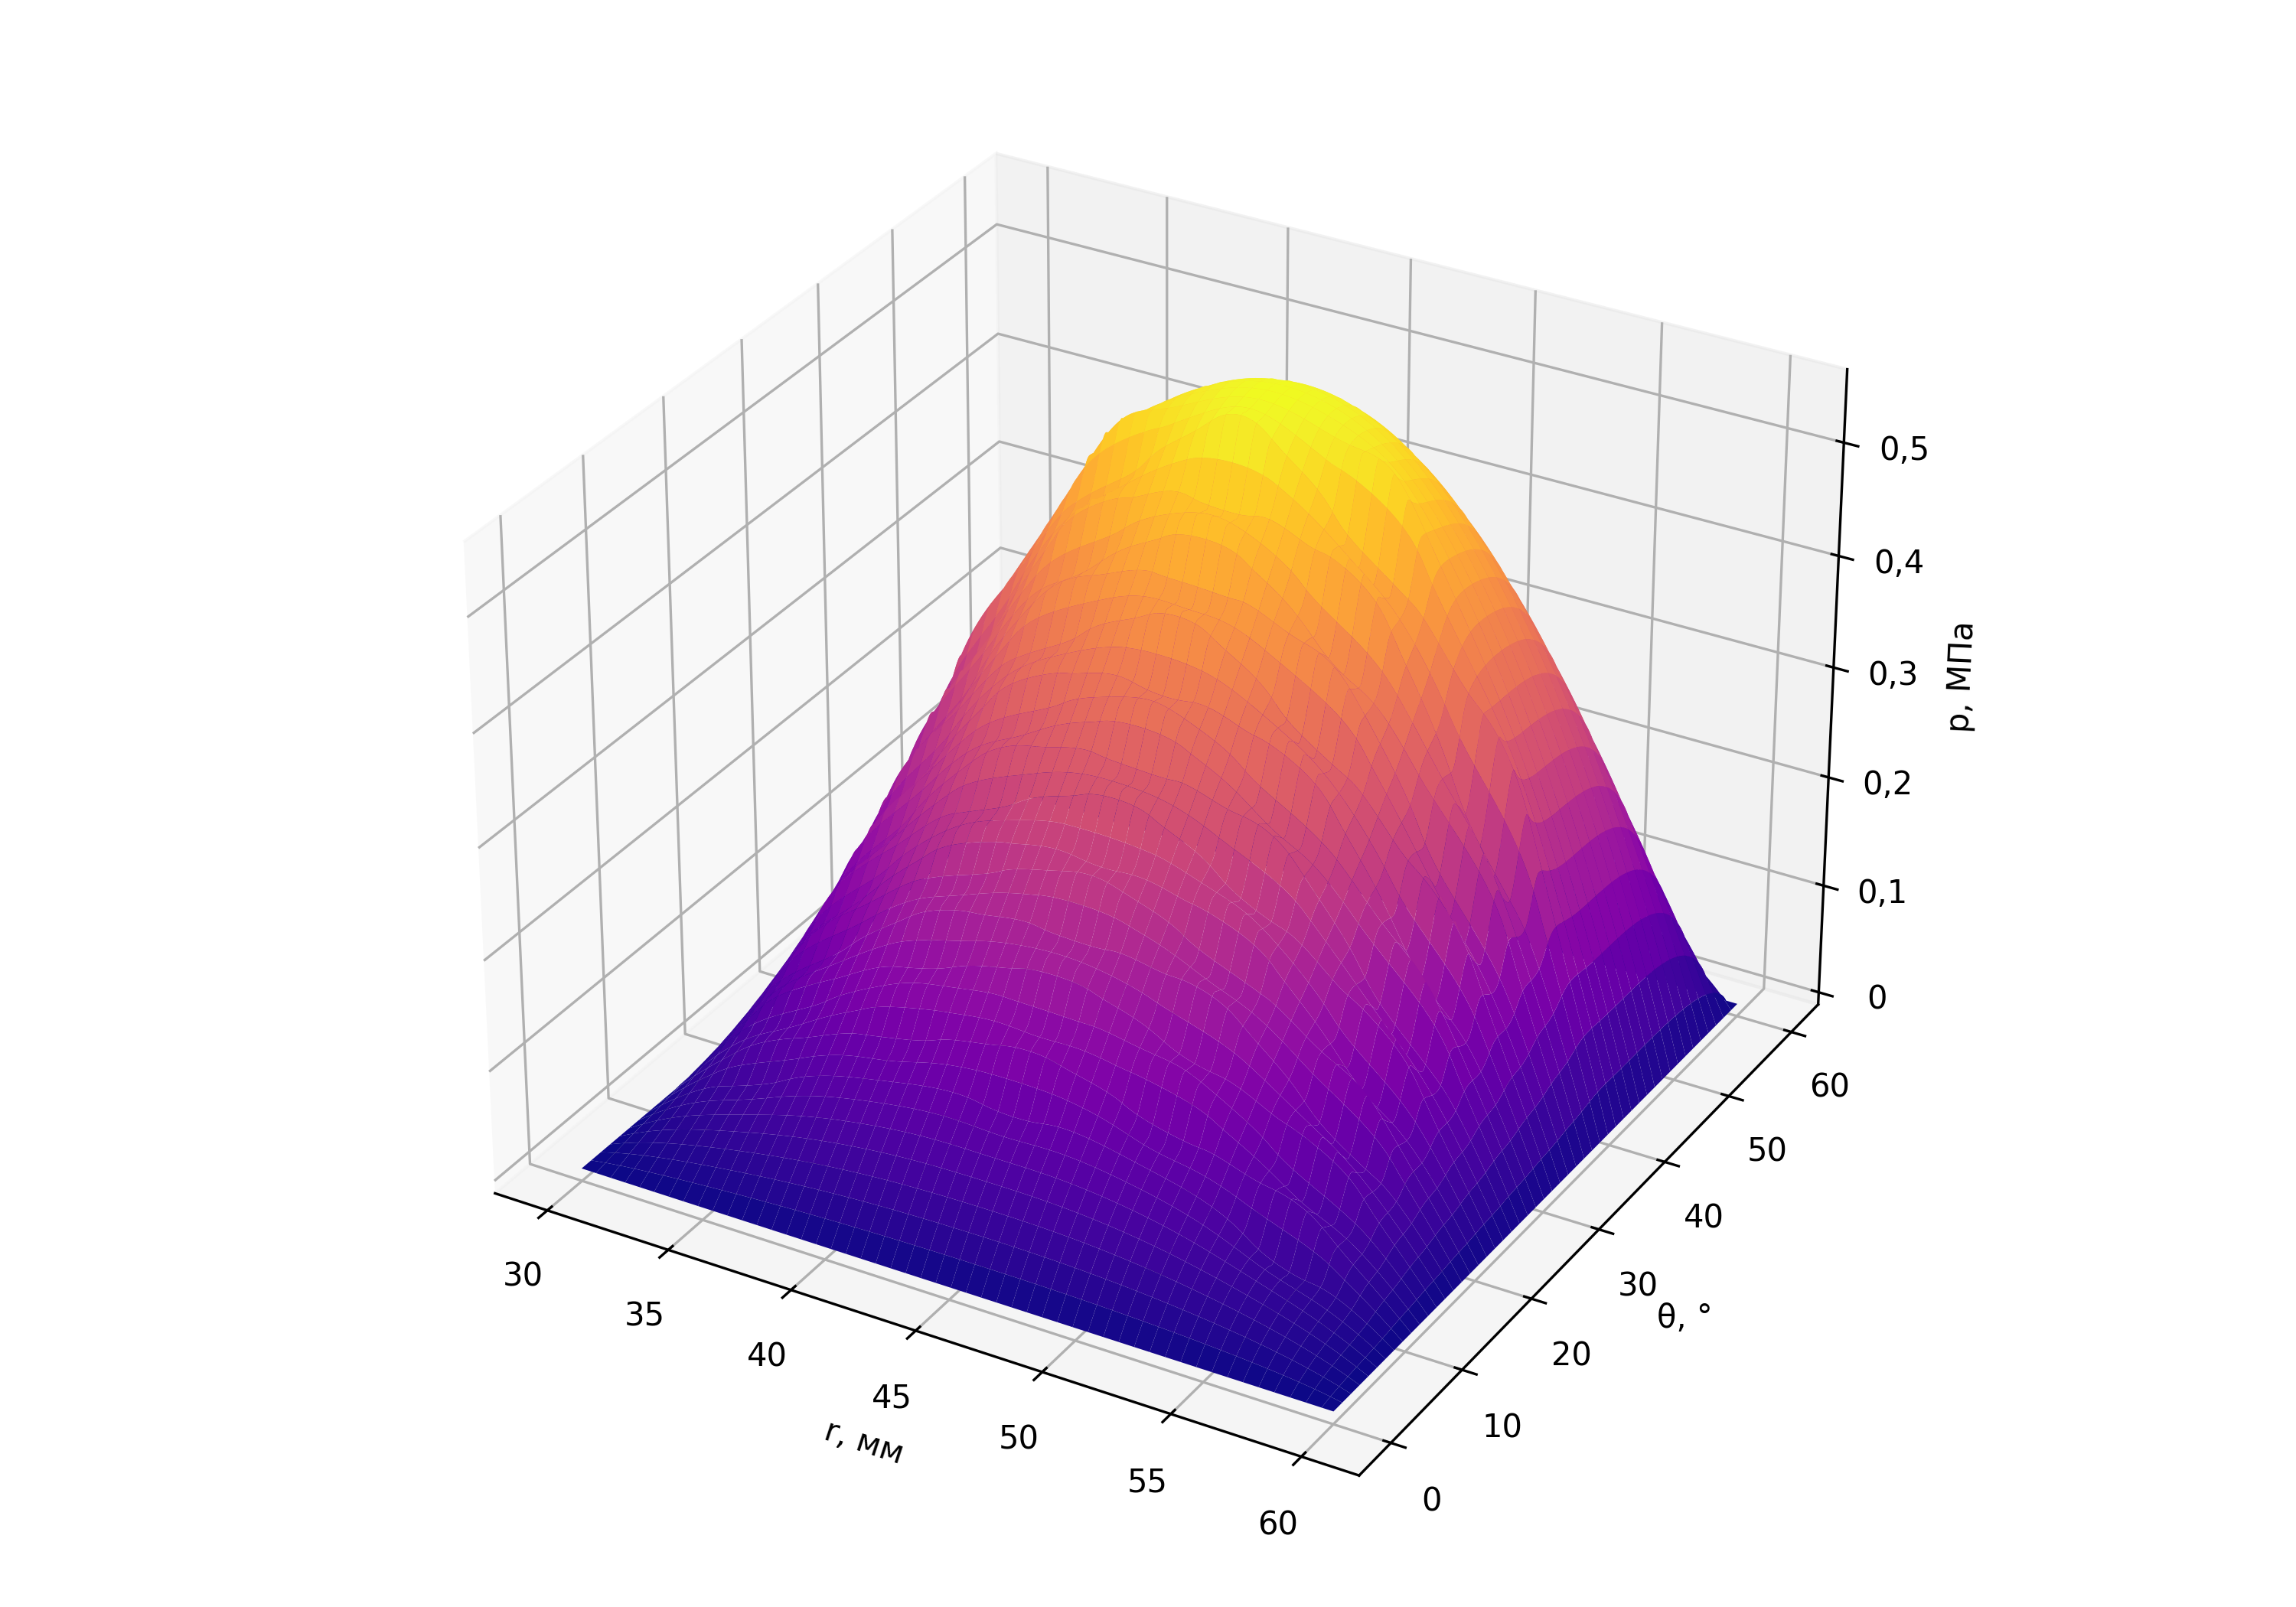
\includegraphics[width=\textwidth,height=0.9\textheight,keepaspectratio]{figures/ch07/fig_7_9.png}
\caption{Поле давления $p(r, \theta)$ для конфигурации~T2
  ($H_p = 0{,}40$, зона $0{,}1\beta$--$0{,}7\beta$)
  при $K_{\mathrm{nom}} = 2{,}0$.}
\label{fig:thrust_P3D_T2}
\end{figure}

\FloatBarrier

\textit{Конфигурация~T3.}
Конфигурация~T3 располагает лунки в средней и выходной части клина,
где зазор мал и давление убывает. В этой зоне передние стенки лунок
не создают эффективного гидродинамического клина; напротив, нарушение
плавности зазора в зоне убывающего давления снижает интегральную
несущую силу ниже уровня гладкого варианта ($G_W = 0{,}9816$).

\FloatBarrier
\section*{Выводы по главе~7}
\phantomsection\addcontentsline{toc}{section}{Выводы по главе~7}

Разработана численная модель упорного подшипника скольжения
с секторными колодками и детерминированными микроструктурами
рабочей поверхности~\cite{suh2015a,suh2015b,yang2021,song2024}. Модель основана на цилиндрической форме
уравнения Рейнольдса~\eqref{eq:thrust_reynolds}, решаемого
методом SOR на равномерной сетке $200 \times 300$ с обнулением
отрицательных давлений.

Проведён сравнительный расчёт гладкого варианта и конфигураций
T1, T2, T3 при $K_{\mathrm{nom}} = 2{,}0$. Установлено, что
текстурирование во входной и средней части клина (T1,~T2)
обеспечивает умеренный рост несущей способности и снижение
коэффициента трения. Наилучшие показатели у конфигурации~T2:
$G_W = 1{,}0145$, $G_{f_T} = 1{,}0337$.

Смещение текстуры в среднюю и выходную часть сектора (T3)
оказывается неэффективным: $G_W = 0{,}9816 < 1$, что подтверждает
определяющую роль зоны нанесения текстуры относительно зоны
нарастания давления.

Рост несущей способности при T1 и~T2 сопровождается увеличением
утечек смазочного материала ($G_Q = 0{,}9847$ и $0{,}9733$)
и максимального давления в плёнке ($G_{p_{\max}} = 0{,}9517$
и $0{,}9228$). Данный компромисс необходимо учитывать при выборе
конфигурации рабочей поверхности.

Параметрический расчёт по
$K \in [1{,}5;\; 4{,}0]$ показал, что несущая сила имеет максимум
при $K \approx 2{,}5$ для всех вариантов; коэффициент трения
монотонно убывает с ростом~$K$. Преимущество~T2 по несущей
способности сохраняется по всему исследованному диапазону~$K$.

Результаты анализа упорного подшипника дополняют результаты
глав~5 и~6, расширяя область применения детерминированных
микроструктур на подшипники с клиновым зазором.
